\chapter{\modif{Évaluation de l'algorithme $S \alpha F$}}

\section{Introduction}

\begin{emodif}
\subsection{Comparaison avec l'état de l'art}
Ce chapitre présente l'évaluation de l'algorithme $S \alpha F$. Il commence par une analyse des ses performances  par rapport à celles des méthodes de l'état de l'art :
\begin{itemize}
\item en binarisation interactive par recherche des contours;
\item en binarisation interactive par recherche des régions ;
\item en segmentation interactive \modif{multiclasse}.
\end{itemize}

Se comparer à ces méthodes est une tâche complexe. Pour la majorité des algorithmes de l'état de l'art, aucune implémentation n'a été mise à disposition par les auteurs, nous contraignant à reproduire leurs conditions de test afin d'obtenir pour $S \alpha F$ des résultats qui pourront être confrontés à ceux obtenus par les autres méthodes. Afin de produire les conditions d'une comparaison équitable, nous avons été amené à répondre aux questions suivantes :
\begin{itemize}
\item \textbf{Quelles sont les données employées ?} Trois ensembles de données de référence -- celui Rother \textit{et al.} \cite{rother2004grabcut}, celui de McGuinness \textit{et al.} \cite{mcguinness2010comparative}  et celui Santner \textit{et al.} \cite{santner2010interactive} -- sont utilisés pour l'évaluation des méthodes de binarisation interactive. Cependant leur utilisation est loin d'être uniforme : à notre connaissance, $S \alpha F$ est le seul algorithme de segmentation interactive évalué sur l'intégralité des trois ensembles. Toutes les autres méthodes sont évaluées au mieux sur deux de ces ensembles, souvent sur un seul et parfois même uniquement sur quelques images de chacun des ensembles. Le tableau \ref{tab:eval:donnerefparalgo} récapitule pour chaque méthode les données utilisées.
\item \textbf{Comment la qualité de la segmentation est-elle évaluée ?} Nous verrons que trois mesures sont utilisées  : l'indice de Jaccard, une mesure floue d'adéquation aux contours et la mesure DICE. Là encore, selon les évaluations conduites, une ou plusieurs de ces mesures sont utilisées.
\item \textbf{Comment la rapidité de la méthode est-elle évaluée ? } Le tableau \ref{tab:eval:tempsparalgo} récapitule les informations dont nous disposons pour chaque méthode. La rapidité d'une méthode peut être évaluée :
\begin{itemize}
\item soit en mesurant le temps nécessaire pour produire une segmentation, une fois les germes donnés -- nous nommons cette durée \textit{temps d'exécution} ;
\item soit, dans le cas d'évaluation permettant à l'utilisateur de venir modifier les germes, en mesurant le temps nécessaire pour aboutir à la segmentation recherchée. Cette durée, que nous nommons \textit{durée de convergence},  inclut le temps requis pour donner les germes, le temps utilisé pour les modifier et les temps d'exécution de la méthode pour chaque segmentation produite, chaque fois que les germes sont mis à jour. Dans certains cas, une durée limite est imposée à l'utilisateur : au delà de ce temps imparti, la modification des germes n'est plus possible. Nous nommons cette durée \textit{temps de convergence maximum}. 
\end{itemize}
\end{itemize}

 
\begin{table}[htb]
\caption{Données de référence utilisées pour l'évaluation des différents algorithmes de l'état de l'art.}
\centering
\begin{tabular}{|l|l|}
\hline
\cellcolor{gris}{Algorithme} & \cellcolor{gris}{Données de références}\\
\hline
Milles \textit{et al.} \cite{mille2015combination} & 10 images de Rother \textit{et al.} \cite{rother2004grabcut}\\
\hline 
Mortensen \textit{et al.} \cite{mortensen1995intelligent}& Rother \textit{et al.} \cite{rother2004grabcut} \\
\hline
Boykov \textit{et al.}  \cite{boykov2001interactive}&  McGuinness \textit{et al.} \cite{mcguinness2010comparative}\\ 
\hline
Salembier \textit{et al.} \cite{salembier2000binary}&  McGuinness \textit{et al.} \cite{mcguinness2010comparative}\\
\hline
Friedland \textit{et al.} \cite{friedland2005siox} &  McGuinness \textit{et al.} \cite{mcguinness2010comparative}\\
\hline
Adams \textit{et al.} \cite{adams1994seeded} &  McGuinness \textit{et al.} \cite{mcguinness2010comparative}\\ 
\hline
Jian \textit{et al.} \cite{jian2016interactive} &  McGuinness \textit{et al.} \cite{mcguinness2010comparative} (en partie) \\
\hline
Santner \textit{et al.} \cite{santner2010interactive}& Santner \textit{et al.} \cite{santner2010interactive} \\
\hline
Müller \textit{et al.} \cite{muller2016robust}& Santner \textit{et al.} \cite{santner2010interactive}\\
\hline
 Changjae \textit{et al.} \cite{Changjae2017Robust} & Rother \textit{et al.} \cite{rother2004grabcut} et 50 images de Santner \textit{et al.} \cite{santner2010interactive}\\
\hline
\end{tabular}
\label{tab:eval:donnerefparalgo}
\end{table}

 
\begin{table}[htb]
\caption{Évaluation de la rapidité des méthodes.}
\centering
\begin{tabular}{|l|p{3cm}|p{3cm}|p{3cm}|}
\hline
\cellcolor{gris}{Algorithme} & \cellcolor{gris}{Temps d’exécution}  & \cellcolor{gris}{Modification des germes}  & \cellcolor{gris}{Temps de convergence maximum} \\
\hline
Milles \textit{et al.} \cite{mille2015combination} & OUI & NON & -- \\
\hline 
Mortensen \textit{et al.} \cite{mortensen1995intelligent}& OUI & OUI & 2 minutes  \\
\hline
Boykov \textit{et al.}  \cite{boykov2001interactive}& OUI & OUI & 2 minutes  \\ 
\hline
Salembier \textit{et al.} \cite{salembier2000binary}& OUI & OUI & 2 minutes  \\
\hline
Friedland \textit{et al.} \cite{friedland2005siox} & OUI & OUI & 2 minutes  \\
\hline
Adams \textit{et al.} \cite{adams1994seeded} & OUI & OUI & 2 minutes  \\
\hline
Jian \textit{et al.} \cite{jian2016interactive} & OUI & OUI & --  \\
\hline
Santner \textit{et al.} \cite{santner2010interactive}& OUI & NON & -- \\
\hline
Müller \textit{et al.} \cite{muller2016robust}& OUI & NON & -- \\
\hline
 Changjae \textit{et al.} \cite{Changjae2017Robust} & OUI & NON & -- \\
\hline
\end{tabular}
\label{tab:eval:tempsparalgo}
\end{table}

\subsection{Analyse des propriétés de $S \alpha F$}

Une fois la comparaison avec les méthodes de l'état de l'art réalisée, nous décrirons un ensemble de tests visant à mettre en exergue des propriétés spécifiques de $S \alpha F$. Tout d'abord, nous évaluerons sa capacité de passage à l'échelle.  Ensuite, nous  étudierons son ergonomie. Enfin, nous conclurons avec deux applications de notre algorithme.

\subsection{Conditions générales des tests réalisés}

Les tests décrits ont été réalisés sur un ordinateur équipé d'un processeur $\nombre{2,6}$ GHz Intel Core i7 et de $16$ Go de mémoire vive. Les images sont sur-segmentées en $3000$ superpixels et le paramètre de compacité de l'algorithme de sur-segmentation SLIC a été fixé à $10$. Nous avons utilisé comme méthode de classification un SVM, au travers de l'implémentation LibSVM avec le noyau suivant :
\modif{
\begin{equation}
\mathcal{F}_{RBF}(x,x') = \exp \left( -  \dfrac{|| x -x'||^{2}}{2\sigma^{2}}\right)
\end{equation}}
où $\sigma$ vaut $4$. Le paramètre \modif{pondérant l’importance des erreurs de classification par rapport
à celle de la largeur de la marge de tolérance au bruit dans les données} est lui aussi fixé à $4$. \modif{Le choix de ces deux paramètres est détaillé dans la section \ref{sec:saf:SelectClassifSup}}.

\end{emodif}
\section{Comparaison avec les méthodes de binarisation interactive par recherche des contours}

Nous avons comparé les performances de $S \alpha F$ à celles de deux méthodes de binarisation interactive par recherche des contours : 
\begin{itemize}
\item la méthode de Milles \textit{et al.} \cite{mille2015combination} ;
\item l'algorithme de Mortensen \textit{et al.} \cite{mortensen1995intelligent}.
\end{itemize}

Aucune implémentation n'étant disponible pour l'algorithme de Milles \textit{et al.} \cite{mille2015combination}, nous avons cherché à reproduire au mieux les expérimentations menées par les auteurs.  Pour l'algorithme \modif{de} Mortensen \textit{et al.} \cite{mortensen1995intelligent}, nous avons utilisé l'implémentation incluse dans le logiciel de manipulation d'images Gimp\footnote{\url{https://www.gimp.org/}}.

\subsection{Méthode de Milles \textit{et al.} }

\subsubsection{Conditions de \modif{test} de Milles \textit{et al.}}

Afin d'évaluer leur méthode, Milles \textit{et al.} utilisent un sous-ensemble de dix images, extraites des données de référence mises à disposition par  Rother \textit{et al.} \cite{rother2004grabcut}. À chaque image, une segmentation de référence est associée, correspondant à un problème de binarisation où l'objet à extraire correspond à une unique composante connexe, sans trou. L'adéquation entre l'objet extrait et la segmentation de référence est quantifiée en utilisant l'indice de Jaccard, converti en pourcentage. Soit $R$ une segmentation de référence et $S$ la segmentation produite par une méthode. 

Soit $R_{O}$ les pixels appartenant à l'objet dans la segmentation de référence et $S_{O}$ ceux attribués à ce même objet dans la segmentation résultat. L'indice de Jaccard mesure la précision pour la classe \emph{objet à extraire} et correspond à la proportion de pixels appartenant à l'objet (à la fois dans la segmentation de référence et dans la segmentation produite) par rapport au nombre total de pixels attribués à l'objet dans l'une ou l'autre des segmentations. En le multipliant par $100$ pour obtenir un pourcentage, nous avons :
\modif{\begin{equation}
\label{eq:acc_o_f}
\mathcal{F}_{Jaccard}(R_{O},S_{O})= 100  \frac{|R_{O} \cap S_{O} |}{|R_{O} \cup S_{O}|} \text{.}
\end{equation}}

Pour chaque image, Milles \textit{et al.} \modif{donnent} le minimum, le maximum, la valeur moyenne et l'écart type obtenus avec les différents ensembles de germes. 

\subsubsection{Interprétation des résultats}

Les tests de Milles \textit{et al.} présentent deux particularités qui compliquent leur analyse. Premièrement, ils ne concernent que dix images. Elles correspondent à des problèmes de binarisation relativement simples où l'objet se détache nettement du fond.

Deuxièmement, Milles \textit{et al.} ont fait le choix d'utiliser des germes générés automatiquement. À partir de la segmentation de référence,  le contour de l'objet à extraire est découpé en $N$ segments de tailles identiques. Pour chaque segment, un germe est prélevé en sélectionnant un pixel de manière aléatoire. Pour chaque image, $20$ ensembles de germes différents sont générés, en faisant varier leur nombre et leur position. Les résultats obtenus par Milles \textit{et al.} dans ces conditions ont été recopiés dans le tableau \ref{eval:tab:resMilles}.


\begin{table}[htb]
\caption{Scores  $\mathcal{F}_{Jaccard}$ minimum, moyen (avec l'écart type) et maximum obtenus par la méthode de Milles \textit{et al.} (extraits de l'article \cite{mille2015combination}).}
\centering
\begin{tabular}{|l|l| l|l|}
\hline
\cellcolor{gris}{Nom de l'image} & \cellcolor{gris}{Minimum} & \cellcolor{gris}{Moyenne}  & \cellcolor{gris}{Maximum}  \\
\hline
BANANA1 & $\nombre{20,0}$ &$\nombre{60,4} \pm \nombre{0,20} $&$\nombre{89,1}$ \\ 
\hline
BANANA2 & $\nombre{0,7}$&$\nombre{47,3} \pm \nombre{0,25}$ &$\nombre{88,3}$  \\
\hline
BANANA3& $\nombre{26,1}$ & $\nombre{62,5} \pm \nombre{0,15}$ &$\nombre{86,6}$\\
\hline
CERAMIC & $\nombre{74,8}$& $\nombre{85,6} \pm \nombre{0,03}$ &$\nombre{89,8}$ \\
\hline
DOLL & $\nombre{72,5}$& $\nombre{80,8} \pm \nombre{0,04}$ &$\nombre{87,7}$  \\
\hline
FLOWER & $\nombre{1,4}$ &$\nombre{88,1} \pm \nombre{0,29}$ &$\nombre{98,2}$ \\
\hline
MUSHROOM & $\nombre{33,0}$ & $\nombre{61,3} \pm \nombre{0,17}$ &$\nombre{91,1}$ \\
\hline
MUSIC & $\nombre{97,3}$ & $\nombre{97,8} \pm \nombre{0,01}$&$\nombre{98,6}$ \\
\hline
SHEEP & $\nombre{4,5}$ & $\nombre{77,0} \pm \nombre{0,18}$&$\nombre{90,2}$ \\
\hline
TEDDY &$\nombre{17,6}$  & $\nombre{74,9} \pm \nombre{0,17}$&$\nombre{96,7}$ \\
\hline
Toutes & $\nombre{0,7}$ & $\nombre{73,5} \pm \nombre{0,23}$&  $\nombre{91,4}$\\
\hline
\end{tabular}
\label{eval:tab:resMilles}
\end{table}

Le tableau \ref{tab:eval:safMilles} montre les résultats obtenus par $S \alpha F$ avec les mêmes images. Les germes ont été donnés manuellement. L'utilisateur disposait d'une durée de deux minutes (maximum) par image pour leur apporter des modifications et améliorer la qualité de la segmentation produite. Le pourcentage moyen de pixels annotés par l'utilisateur est égal à $\nombre{0,56} \%$ des pixels de l'image. Les figures \ref{fig:eval:BinC1}, \ref{fig:eval:BinC2} et \ref{fig:eval:BinC3} présentent les germes données à $S \alpha F$  et les segmentations réalisées. 

\begin{table}[htb]
\caption{Scores  $\mathcal{F}_{Jaccard}$ obtenus par la méthode $S \alpha F$.}
\centering
\begin{tabular}{| l |l |}
\hline
\cellcolor{gris}{Nom de l'image} & $\cellcolor{gris}{S \alpha F }$ \\
\hline
BANANA1 & $\nombre{97,1}$\\ 
\hline
BANANA2   & $\nombre{96,4}$\\
\hline
BANANA3 &  $\nombre{97,9}$\\
\hline
CERAMIC   &  $\nombre{97,5}$\\
\hline
DOLL  & $\nombre{98,9}$\\
\hline
FLOWER  & $\nombre{98,6}$\\
\hline
MUSHROOM  &$\nombre{97}$\\
\hline
MUSIC & $\nombre{98,9}$\\
\hline
SHEEP   & $\nombre{96,2}$\\
\hline
TEDDY  & $\nombre{95,8}$\\
\hline
Tous  & $\nombre{97,2}$\\
\hline
\end{tabular}
\label{tab:eval:safMilles}
\end{table}


Au vu des conditions de \modif{test} décrites précédemment\modif{,} il n'est pas possible de comparer strictement les deux méthodes. D'une part la méthode de Milles \textit{et al.} utilise des germes bien plus précis (ce sont des points de contour) que ceux de $S \alpha F$. D'autre part, les germes de $S \alpha F$ ont été modifiés par l'utilisateur durant le processus de segmentation. 

Avec moins de trois itérations (donc de trois modifications des germes),  $S \alpha F$ obtient des résultats très satisfaisants. Par ailleurs, alors que le temps d'exécution de la méthode de Milles \textit{et al.} dépend à la fois du nombre de pixels et du nombre de germes, celui de $S \alpha F$ est relié uniquement au nombre de pixels durant l'étape d'initialisation et au nombre de superpixels durant l'étape de segmentation. Ainsi, tandis que l'algorithme de Milles \textit{et al.} affiche des temps de calcul allant de $3$ à $17$ secondes pour produire une segmentation une fois que les germes ont été donnés, le temps d'exécution de $S \alpha F$ pour réaliser la même tâche est de seulement $\nombre{0,6}$ \modif{seconde}, dans des conditions matérielles équivalentes.

\begin{figure}[htb]
	\centering	
	 \begin{subfigure}[B]{0.7\textwidth}	
			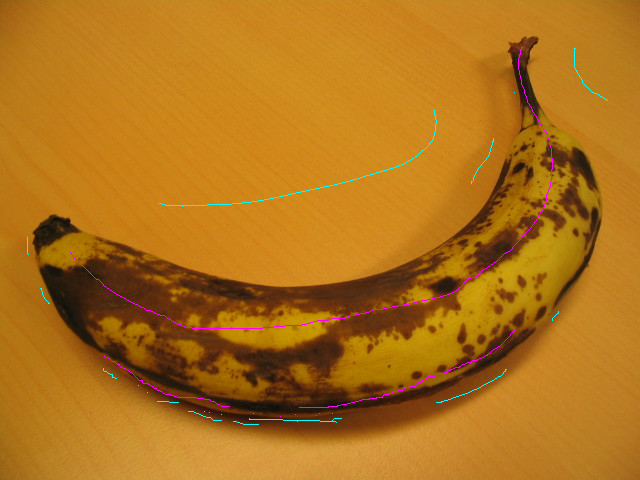
\includegraphics[width=0.45\textwidth]{images/evaluation/Milles/banana1_seeds.jpg}
			
\includegraphics[width=0.45\textwidth]{images/evaluation/Milles/banana1_seg.png}
		 \caption{Image BANANA1.}
	\end{subfigure}		
	\\	
	 \begin{subfigure}[B]{0.7\textwidth}	
			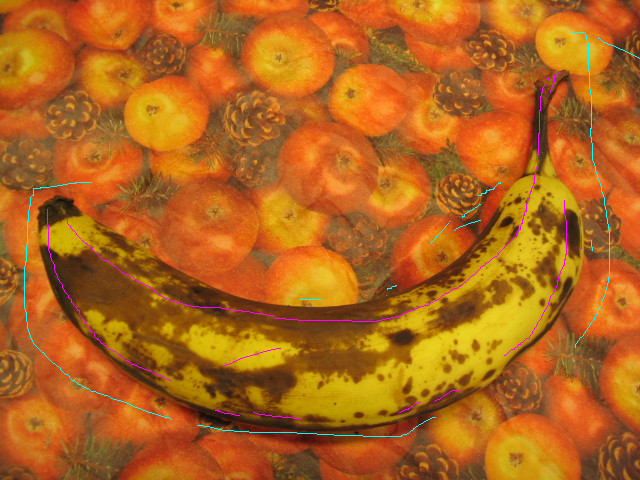
\includegraphics[width=0.45\textwidth]{images/evaluation/Milles/banana2_seeds.jpg}
			
\includegraphics[width=0.45\textwidth]{images/evaluation/Milles/banana2_seg.png}
		 \caption{Image BANANA2.}
	\end{subfigure}		
	\\	
	 \begin{subfigure}[B]{0.7\textwidth}	
			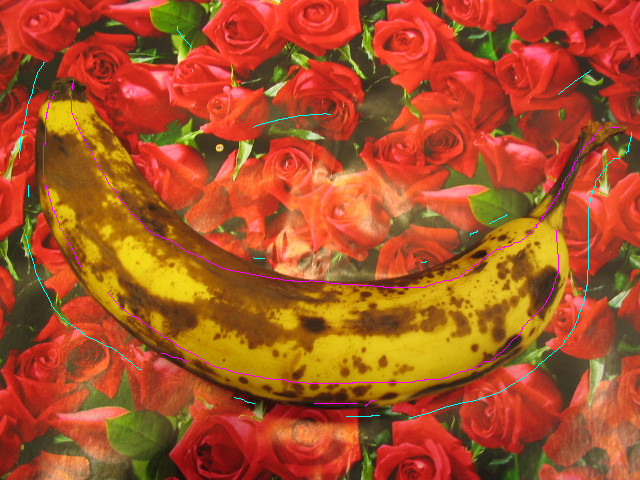
\includegraphics[width=0.45\textwidth]{images/evaluation/Milles/banana3_seeds.jpg}
			
\includegraphics[width=0.45\textwidth]{images/evaluation/Milles/banana3_seg.png}
		 \caption{Image BANANA3.}
	\end{subfigure}		
	\\
	 \begin{subfigure}[B]{0.7\textwidth}	
			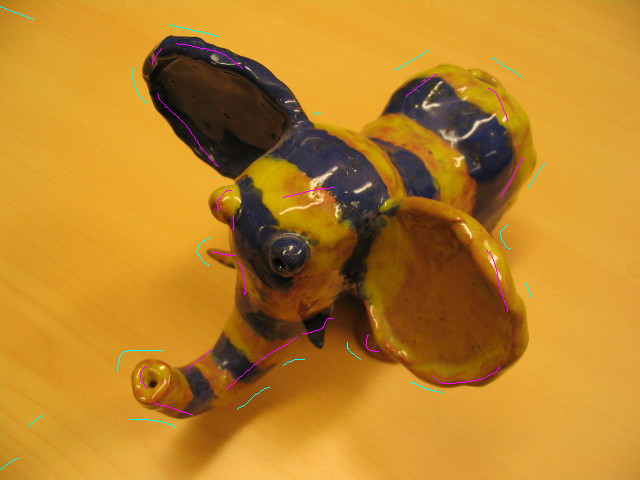
\includegraphics[width=0.45\textwidth]{images/evaluation/Milles/ceramic_seeds.jpg}
			
\includegraphics[width=0.45\textwidth]{images/evaluation/Milles/ceramic_seg.png}
		 \caption{Image CERAMIC.}
	\end{subfigure}	
	\caption{Germes donnés et \modif{segmentations} produites par $S \alpha F$, pour les images utilisées lors des tests de Milles \textit{et al.}}
	\label{fig:eval:BinC1}
\end{figure}

\begin{figure}[htb]
	\centering	
	 \begin{subfigure}[B]{0.7\textwidth}	
			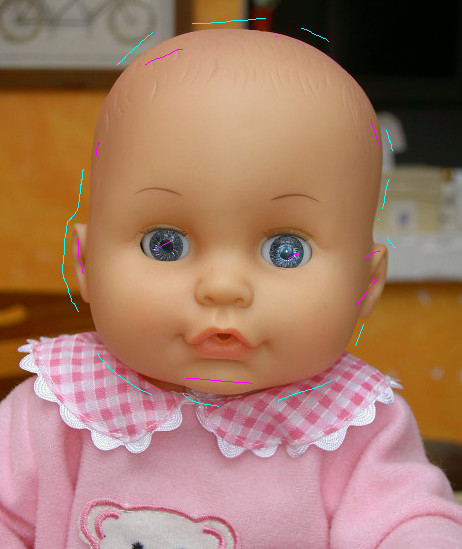
\includegraphics[width=0.45\textwidth]{images/evaluation/Milles/doll_seeds.jpg}
			
\includegraphics[width=0.45\textwidth]{images/evaluation/Milles/doll_seg.png}
		 \caption{Image DOLL.}
	\end{subfigure}	
	\\
	 \begin{subfigure}[B]{0.7\textwidth}	
			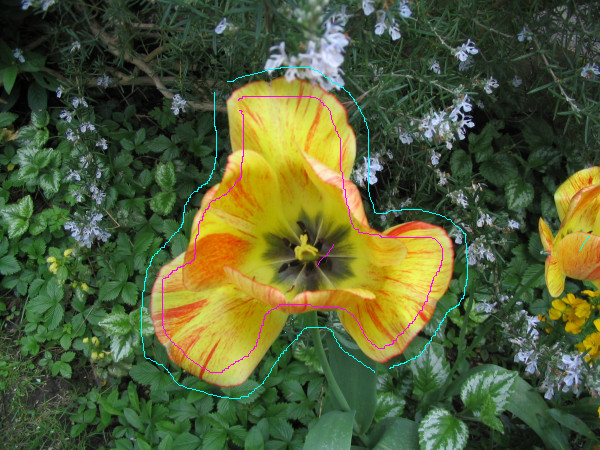
\includegraphics[width=0.45\textwidth]{images/evaluation/Milles/flower_seeds.jpg}
			
\includegraphics[width=0.45\textwidth]{images/evaluation/Milles/flower_seg.png}
		 \caption{Image FLOWER.}
	\end{subfigure}	
	\\
	 \begin{subfigure}[B]{0.7\textwidth}	
			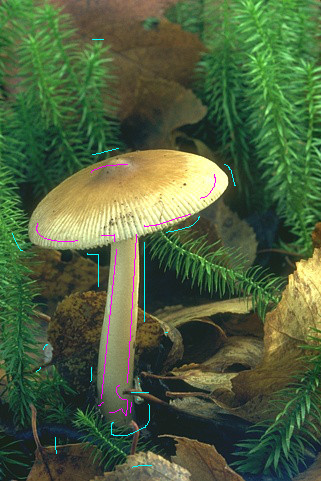
\includegraphics[width=0.45\textwidth]{images/evaluation/Milles/208001_seeds.jpg}
			
\includegraphics[width=0.45\textwidth]{images/evaluation/Milles/208001_seg.png}
		 \caption{Image MUSHROOM.}
	\end{subfigure}	
	\caption{Germes donnés et \modif{segmentations} produites par $S \alpha F$, pour les images utilisées lors des tests de Milles \textit{et al.} (suite).}
	\label{fig:eval:BinC2}
\end{figure}

\begin{figure}[htb]
	\centering	
	 \begin{subfigure}[B]{0.7\textwidth}	
			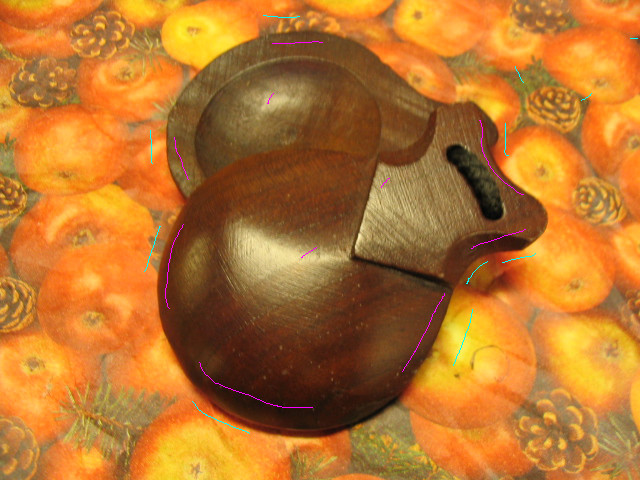
\includegraphics[width=0.45\textwidth]{images/evaluation/Milles/music_seeds.jpg}
			
\includegraphics[width=0.45\textwidth]{images/evaluation/Milles/music_seg.png}
		 \caption{Image MUSIC.}
	\end{subfigure}	
	\\
	 \begin{subfigure}[B]{0.7\textwidth}	
			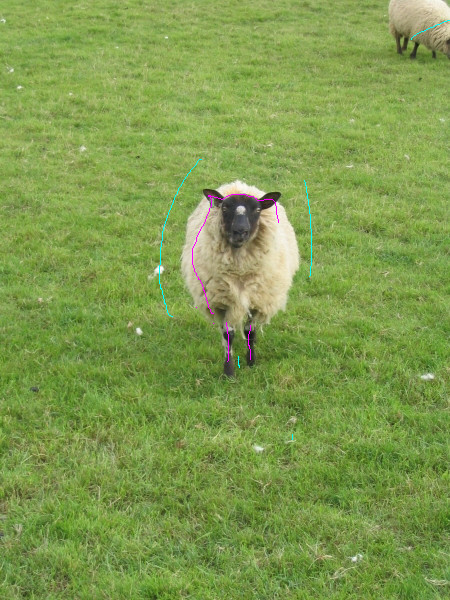
\includegraphics[width=0.45\textwidth]{images/evaluation/Milles/sheep_seeds.jpg}
			
\includegraphics[width=0.45\textwidth]{images/evaluation/Milles/sheep_seg.png}
		 \caption{Image SHEEP.}
	\end{subfigure}	
	\\
	 \begin{subfigure}[B]{0.7\textwidth}	
			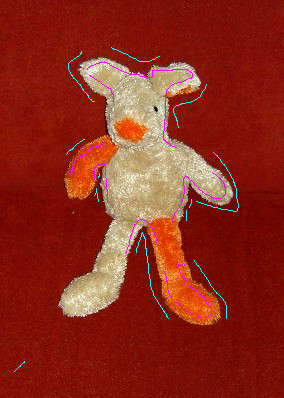
\includegraphics[width=0.45\textwidth]{images/evaluation/Milles/teddy_seeds.jpg}
			
\includegraphics[width=0.45\textwidth]{images/evaluation/Milles/teddy_seg.png}
		 \caption{Image TEDDY.}
	\end{subfigure}	
	\caption{Germes donnés et \modif{segmentations} produites par $S \alpha F$, pour les images utilisées lors des tests de Milles \textit{et al.} (fin).}
	\label{fig:eval:BinC3}
\end{figure}



\subsection{Méthode de Mortensen \textit{et al.}}


Comme nous disposions d'une implémentation de l'algorithme de Mortensen \textit{et al.} \modif{\cite{mortensen1995intelligent}}, nous avons réalisé des tests sur les données de référence de Rother \textit{et al.} \cite{rother2004grabcut}. \modif{Les autres ensembles de données de référence ne sont pas adaptés à l'évaluation de méthodes de binarisation interactive par recherche des contours, qui visent à extraire un unique objet correspondant à une surface sans trou. En effet, soient ils contiennent plus de deux classes, soit les objets sont composés de plusieurs composantes connexes ou d'une composante connexe avec des trous.}  Pour la méthode de Mortensen \textit{et al.}\modif{,} comme pour $S \alpha F$, les germes sont donnés manuellement. \modif{Le temps maximal de convergence est de $2$ minutes : au delà de cette durée l'utilisateur n'est plus autorisé à modifier les germes. En pratique, pour la totalité des images et les deux algorithmes, le temps de convergence est de quelques secondes.}

La méthode de Mortensen \textit{et al.}  obtient un score $\mathcal{F}_{Jaccard}$ de $\nombre{94,5}\%$. L'algorithme $S \alpha F$ permet une amélioration de pratiquement $2 \%$, avec un score de $\nombre{96,3}\%$.

En termes de temps d’exécution, sur les images traitées, les deux méthodes fonctionnent en temps interactif, avec un temps d'exécution inférieur à $1$ seconde. 


\section{Comparaison avec les méthodes de binarisation \modif{interactive} par recherche des régions }

\subsection{Protocole expérimental de McGuinness \textit{et al.}}
L'étude menée en 2010 par McGuinness \textit{et al.} \cite{mcguinness2010comparative} est, à notre connaissance, l'évaluation la plus complète concernant le problème de la binarisation interactive. Elle analyse les performances de quatre algorithmes, proposés respectivement par Boykov \textit{et al.}  \cite{boykov2001interactive},  Salembier \textit{et al.} \cite{salembier2000binary},  Friedland \textit{et al.} \cite{friedland2005siox} et Adams \textit{et al.} \cite{adams1994seeded}\footnote{\modif{L'algorithme d'Adams \textit{et al.} \cite{adams1994seeded} permet aussi de résoudre des problèmes multiclasses.}}. 

À partir des images de la base de données de Berkeley \cite{MartinFTM01}, McGuinness \textit{et al.} \modif{ont créé} un ensemble de données de référence totalisant $96$ images et $100$ segmentations de référence. Chaque segmentation de référence correspond à un problème de binarisation où un objet doit être extrait du fond. Ainsi, lorsqu'une image contient plusieurs objets intéressants, plusieurs segmentations de référence lui sont associées. Les objets peuvent contenir des trous ou être constitués de plusieurs régions. 

De petite taille ($481 \times 321$ pixels), les photographies utilisées comprennent malgré tout de nombreux détails, restitués avec précision dans les segmentations de référence. La figure \ref{fig:eval:MgDBEx}a en fournit un exemple. En outre, les objets à extraire n'occupent pas nécessairement la majorité de l'image, comme dans le cas du dromadaire de la figure \ref{fig:eval:MgDBEx}b. Tous ces aspects contribuent à faire des données de référence de McGuinness \textit{et al.} un ensemble de problèmes de binarisation difficiles.

\modif{Les tests mis en place par McGuinness \textit{et al.} font intervenir un panel d'utilisateurs, testant chacune des méthodes en lui donnant manuellement des germes}. Afin d'aboutir à une segmentation la plus proche possible de chaque segmentation de référence, McGuinness \textit{et al.} autorisent l'utilisateur à ajouter ou supprimer autant de germes que nécessaire, durant au plus deux minutes \modif{(il s'agit de ce que nous nommons le temps maximal de convergence)}.  Au delà de cette durée, l'utilisateur n'est plus autorisé à modifier les germes. Ce temps ne doit pas être confondu avec le temps d'exécution nécessaire à un algorithme pour produire une segmentation une fois les germes donnés.

\begin{figure}[htb]
	\centering	
	 \begin{subfigure}[B]{\textwidth}
	 \centering
			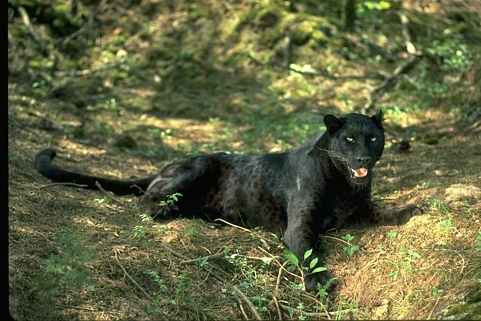
\includegraphics[width=0.45\textwidth]{images/evaluation/McGuinness/304034.jpg}
			
\includegraphics[width=0.45\textwidth]{images/evaluation/McGuinness/304034.png}
		 \caption{Problème de segmentation où le fond comprend de petits éléments, complexes à extraire.}
	\end{subfigure}		
	\\	
	 \begin{subfigure}[B]{\textwidth}	
	 \centering
			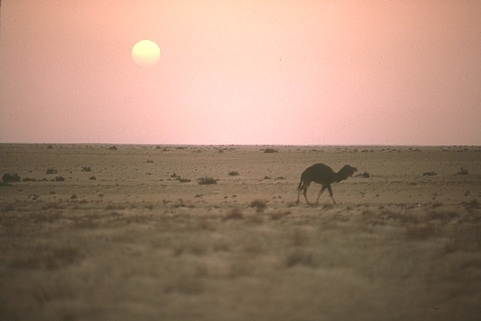
\includegraphics[width=0.45\textwidth]{images/evaluation/McGuinness/271031.jpg}
			
\includegraphics[width=0.45\textwidth]{images/evaluation/McGuinness/271031.png}
		 \caption{Problème de segmentation où l'objet à extraire est très petit par rapport au fond.}
	\end{subfigure}	
	\caption{Exemples d'images (à gauche) et de segmentations de référence (à droite) mises à disposition par McGuinness \textit{et al.} \cite{mcguinness2010comparative}.}
	\label{fig:eval:MgDBEx}
\end{figure}


À la fin des tests, la qualité des \modif{segmentations} est évaluée grâce à deux mesures : l'indice de Jaccard \modif{$\mathcal{F}_{Jaccard}$, }présenté dans la section précédente et une mesure floue d'adéquation aux contours, \modif{$\mathcal{F}_{Cnt}$}.

Soit $R$  une segmentation de référence et $S$  une segmentation produite par une méthode de segmentation interactive. Comme nous nous intéressons à des problèmes de binarisation, les segmentations $R$ et $S$ donnent chacune une partition de l'image en deux ensembles :
\begin{itemize}
\item $R_{O}$ et $R_{F}$, qui séparent les pixels de l'objet des pixels du fond dans la segmentation de référence ;
\item $S_{O}$ et $S_{F}$, qui séparent les pixels de l'objet des pixels du fond dans la segmentation résultat.
\end{itemize}

Un pixel appartenant à l'un des ensembles et ayant un de ses voisins dans un autre ensemble, constitue un point de contour. McGuinness \textit{et al.} souhaitent vérifier que les contours dans $S$ suivent les contours dans $R$.

Soit $C_{R}$  l'ensemble des points de contour de $R$ et $C_{S}$ l'ensemble des points de contours de $S$. \modif{La mesure  suivante, quantifie l'adéquation entre les contours dans $R$ et ceux dans $S$ :}
\modif{\begin{equation}
\mathcal{F}_{Cnt} = \dfrac{| C_{R} \cap  C_{S} |}{| C_{R} \cup  C_{S} |}\text{.}
\end{equation}}

L'un des inconvénients de cette mesure est qu'elle ne prend en compte aucune marge d'erreur :  les pixels des contours doivent coïncider parfaitement. L'idée de McGuinness \textit{et al.} consiste à étendre les ensembles $C_{R}$ et $C_{S}$ à l'aide de la théorie des \modif{sous-ensembles} flous, afin de permettre que deux pixels de contour proches \modif{l'un de l'autre} contribuent également à améliorer le score. 

Ainsi, pour un pixel $p_{i}$ de l'image, son degré d'appartenance à un contour d'une segmentation S est donné par la fonction gaussienne :
\modif{\begin{equation}
\mathcal{F}_{App}(p_{i},S) = \exp \left( - \dfrac{||p_{i} - p_{j} ||} {\sigma^{2}} \right)
\end{equation}}
où
\begin{itemize}
\item $|| p_{i} - p_{j}||$ est \modif{la distance euclidienne} entre les pixels $p_{i}$ et $p_{j}$ ;
\item $\displaystyle p_{j} = \argmin_{p_{k} \in C_{S}} ||p_{i}-p_{k}||$ est le pixel\modif{,} appartenant \modif{à} un contour\modif{,} le plus proche de $p_{i}$ ;
\item $\sigma$ est un paramètre permettant de régler le seuil de tolérance ; McGuinness \textit{et al.} proposent de le fixer à  $4$.
\end{itemize}
La mesure d'adéquation \modif{aux} contours, exprimée en pourcentage, devient alors :
\modif{\begin{equation}
\mathcal{F}_{FCnt} = 100 \dfrac{ \displaystyle  \sum_{i=1}^{N_{I}} \min(\mathcal{F}_{App}(p_{i},S) , \mathcal{F}_{App}(p_{i},R) )}{ \displaystyle \sum_{i=1}^{N_{I}} \max(\mathcal{F}_{App}(p_{i},S) , \mathcal{F}_{App}(p_{i},R) )}\text{.}
\end{equation}}

Pour chacune de ces deux mesures, \modif{$\mathcal{F}_{Jaccard} $ et $\mathcal{F}_{FCnt} $} les scores moyens obtenus sur l'ensemble des images sont donnés.

\subsection{Méthodes testées par McGuinness \textit{et al.}}

Le tableau \ref{tab:eval:resbinreg1} résume les scores obtenus par les algorithmes de  Boykov \textit{et al.}  \cite{boykov2001interactive}, \modif{de} Salembier \textit{et al.} \cite{salembier2000binary}, de Friedland \textit{et al.} \cite{friedland2005siox} et d'Adams \textit{et al.} \cite{adams1994seeded} lors de l'évaluation réalisée par McGuinness \textit{et al.} \cite{mcguinness2010comparative}. Il donne également les scores atteints par $S \alpha F$ dans des conditions expérimentales similaires. \modif{Le temps maximum de convergence, de deux minutes par image, a été respecté. Dans la majorité des cas, le temps réel de convergence pour $S \alpha F$ est bien inférieur : de quelques secondes pour les images les plus simples et jusqu'à une minute, pour la majorité des images.}

\begin{table}[H]
\caption{Comparaison de $S \alpha F$ avec les méthodes évaluées par McGuinness \textit{et al.}}
\centering
\begin{tabular}{|l|l|l|}
\hline
\cellcolor{gris}{Algorithme} & $\cellcolor{gris}{\mathcal{F}_{Jaccard}}$ & $\cellcolor{gris}{\mathcal{F}_{FCnt}}$ \\
\hline
Boykov \textit{et al.}& $92$ & $77$ \\
\hline
Salembier \textit{et al.}& $92$ & $78$ \\
\hline
Friedland \textit{et al.}& $85$ & $64$ \\
\hline
Adams \textit{et al.}& $88$ & $70$ \\
\hline
$S \alpha F$& ${95}$ & ${83}$ \\
\hline
\end{tabular}
\label{tab:eval:resbinreg1}
\end{table}

\modif{Les résultats du tableau \ref{tab:eval:resbinreg1}} montrent que les segmentations produites par $S \alpha F$ sont plus proches des segmentations de référence que celles des autres algorithmes. En particulier, le score de $S \alpha F$ est supérieur de $2\%$ à celui obtenu par les méthodes de Boykov \textit{et al.} et de Salembier \textit{et al.} pour la mesure $\mathcal{F}_{Jaccard}$ et de plus de $5\%$ pour la mesure $\mathcal{F}_{FCnt}$. Ils indiquent que, malgré l'utilisation des superpixels, $S \alpha F$ réussit à extraire précisément les détails contenus dans les images. \modif{C}es résultats ont été obtenus avec des temps d'exécution autour de $\nombre{0,7}$ seconde, ce qui est similaire aux temps d'exécution des méthodes comparées. La figure \ref{fig:eval:ResMG} illustre par quelques exemples le comportement de $S \alpha F$.

\begin{figure}[htb]
	\centering	
	 \begin{subfigure}[B]{\textwidth}
	 \centering
			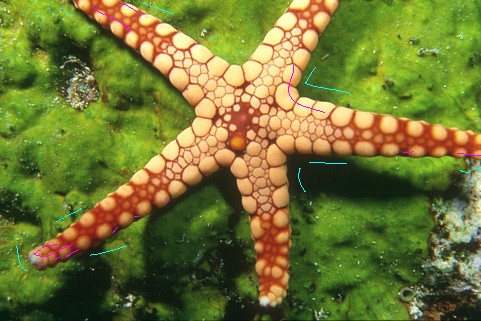
\includegraphics[width=0.45\textwidth]{images/evaluation/McGuinness/12003_seeds.jpg}
			
\includegraphics[width=0.45\textwidth]{images/evaluation/McGuinness/12003_seg.png}
		 \caption{Objet fortement contrasté avec le fond : l'utilisation d'une information de couleur permet d'obtenir une segmentation précise à l'aide de seulement quelques germes.}
	\end{subfigure}		
	\\	
	 \begin{subfigure}[B]{\textwidth}	
	 \centering
			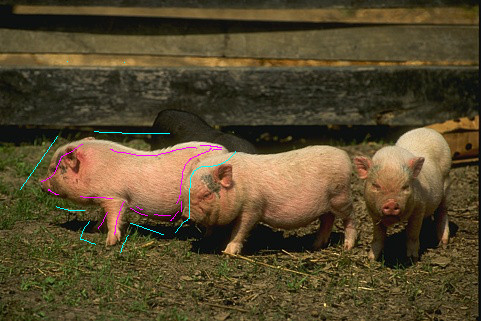
\includegraphics[width=0.45\textwidth]{images/evaluation/McGuinness/66053_seeds.jpg}
			
\includegraphics[width=0.45\textwidth]{images/evaluation/McGuinness/66053_seg.png}
		 \caption{Image où l'objet à extraire est très similaire à une partie du fond : l'information de localisation permet malgré tout d'obtenir une segmentation précise.}
	\end{subfigure}	
	\\	
	 \begin{subfigure}[B]{\textwidth}	
	 \centering
			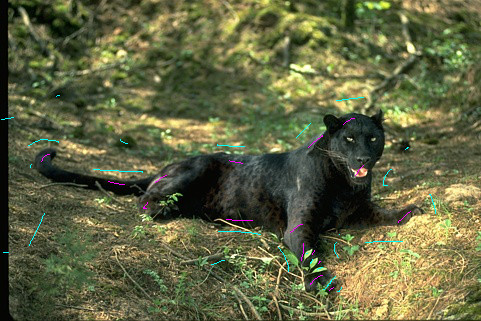
\includegraphics[width=0.45\textwidth]{images/evaluation/McGuinness/304034_seeds.jpg}
			
\includegraphics[width=0.45\textwidth]{images/evaluation/McGuinness/304034_seg.png}
		 \caption{Image où le fond comprend de petits éléments difficiles à extraire.}
	\end{subfigure}	
	\caption{Exemples de germes donnés et de résultats obtenus \modif{par $S \alpha F$} sur les données de référence de McGuinness \textit{et al.} }
	\label{fig:eval:ResMG}
\end{figure}

 Sur l'image de la figure \ref{fig:eval:ResMG}a, l'objet à extraire est nettement distinguable du fond. L'utilisation d'une information de couleur permet d'obtenir une segmentation correcte avec très peu de germes. Au contraire, l'objet à extraire de la figure \ref{fig:eval:ResMG}b est l'un des trois porcelets blancs. L'information de couleur n'est donc pas suffisante pour l'isoler. Ici, c'est l'information de localisation qui permet d'obtenir la segmentation désirée. Enfin, la figure \ref{fig:eval:ResMG}c correspond à l'un des exemples d'images comprenant de petits détails et qui a été présentée précédemment. 

\subsection{Algorithme de Jian \textit{et al.}}
Nous n'avons malheureusement pas pu réaliser une comparaison rigoureuse entre $S \alpha F$ et la méthode de binarisation interactive par recherche des régions la plus récente, proposé par Jian \textit{et al.} \cite{jian2016interactive}. En effet, les auteurs affirment avoir utilisé comme données d'évaluation une version étendue de l'ensemble de données de référence de McGuinness \textit{et al.}, sans la mettre à disposition. Nous soulignerons toutefois que
les performances atteintes par $S \alpha F$ sur les images de McGuinness \textit{et al.} correspondent à une amélioration de $2 \%$\footnote{Ce pourcentage correspond à la différence obtenue pour la mesure $\mathcal{F}_{Jaccard}$, Jian \textit{et al.} n'ayant pas communiqué de chiffres pour la mesure $\mathcal{F}_{FCnt}$.} par rapport à l'algorithme de Jian \textit{et al.} Les temps d'exécution de $S \alpha F$ sont supérieurs de quelques dixièmes de secondes.


\section{Comparaison avec les méthodes de \modif{segmentation interactive multiclasse}}

Nous avons comparé $S \alpha F$ à trois méthodes de \modif{segmentation multiclasse} : celle de Santner \textit{et al.} \cite{santner2010interactive}, celle de \modif{Müller} \textit{et al.} \cite{muller2016robust}  et celle de Changjae \textit{et al.} \cite{Changjae2017Robust}. 
\subsection{Données utilisées}

Ces trois méthodes ont été évaluées avec les données de référence de Santner \textit{et al.}, qui comprennent $158$ photographies de $625 \times 391$ pixels et $262$ segmentations de référence, pour des problèmes \modif{multiclasses}.  La figure \ref{fig:eval:stnerClasses} donne la répartition du nombre de classes pour ces segmentations. Elle montre qu'une majorité des problèmes posés comprennent entre 2 et 4 classes. 

\begin{figure}[htb]
\begin{center}
\scalebox{.4}{
\input{images/evaluation/santernClasses.pdf_t}
}
\caption{Répartition du nombre de classes pour les données de référence mises à disposition par Santner \textit{et al.} \cite{santner2010interactive}.}
\label{fig:eval:stnerClasses}
\end{center}
\end{figure}

\subsection{Mesure de la précision d'une segmentation}

Afin d'évaluer l'adéquation entre une segmentation de référence $R$ et une segmentation produite $S$, Santner \textit{et al.},  \modif{Müller} \textit{et al.} et Changjae \textit{et al.} utilisent la mesure $\mathcal{F}_{DICE}$ \cite{santner2010interactive}, dont la valeur convertie en pourcentage vaut :
\begin{equation}
\label{eq:dice}
\mathcal{F}_{DICE} = 100 \sum_{i=1}^{N_{\Lambda}} 2 \frac{|R_{i} \cap S_{i} |}{|R_{i} \cup S_{i}|}\text{.}
\end{equation}
Les ensembles $R_{i}$ et $S_{i}$ correspondent à l'ensemble des pixels de label $\lambda_{i}$, respectivement dans la segmentation de référence et dans la segmentation produite. Santner \textit{et al.}, \modif{Müller} \textit{et al.} et Changjae \textit{et al.} donnent les scores $\mathcal{F}_{DICE}$ moyens obtenus par leurs méthodes pour l'ensemble des images testées.


\subsection{Méthodes de Santner \modif{\textit{et al.}} et de \modif{Müller} \textit{et al.}}

En plus des données de référence\modif{,} Santner \textit{et al.} \cite{santner2010interactive} ont mis à disposition les germes utilisés par leur méthode. Ces germes ont été \modif{donnés} à l'aveugle, c'est-à-dire sans voir le résultat produit par la méthode de segmentation interactive. En utilisant ces germes, leur méthode obtient un score $DICE$ moyen de $93$. Celle de \modif{Müller} \textit{et al.} \cite{muller2016robust} atteint $94$.


\subsubsection{Résultats avec les germes de Santner \textit{et al.}}

Avec les germes de Santner \textit{et al.}, $S \alpha F$ obtient \modif{de mauvais résultats}, avec un score \modif{$\mathcal{F}_{DICE}$} moyen \modif{de $83 \%$}.  Pour cette mesure, l'écart type est élevé ($14 \%$). L'analyse de l'histogramme des résultats obtenus pour \modif{l'ensemble} des images montre que :
\begin{itemize}
\item pour $ 32  \%$ des couples (germes,  \modif{image}) le score \modif{$\mathcal{F}_{DICE}$} se situe entre $94$ et $99$ ; 
\item pour \modif{$35\%$} des couples (germes,  \modif{image}) le score \modif{$\mathcal{F}_{DICE}$} se situe entre $80$ et $93$ ; 
\item pour \modif{$33\%$} des couples (germes,  \modif{image}) le score \modif{$\mathcal{F}_{DICE}$} se situe entre 40 et \modif{$79$}.
\end{itemize}

Pour \modif{$67\%$} des données, nous obtenons donc des résultats \modif{\og \textit{normaux \fg}} (compris entre $80$ et $99$). L'étude des \modif{$33\%$} de données aboutissant à des segmentations fortement erronées permet de mieux comprendre les limites de $S \alpha F$. 

Les figures \ref{fig:eval:seedsSantner1} et \ref{fig:eval:seedsSantner2} donnent deux exemples où les germes de Santner \textit{et al.} ne permettent pas \modif{à} $S \alpha F$ de produire une segmentation adéquate. Elles comprennent également un exemple, où, avec des germes différents, une segmentation bien meilleure est obtenue. L'étude de la différence entre les deux types de germes montre que pour que $S \alpha F$ produise une segmentation pertinente les germes doivent \modif{positionnés près des contours} des différents objets. 

Dans certains cas, comme \modif{avec} l'exemple de la figure \ref{fig:eval:seedsSantner1}, cela implique \modif{de donner des germes plus nombreux que ceux} de Santner \textit{et al.} Dans de nombreux autres cas, à l'instar de l'exemple présenté sur la figure \ref{fig:eval:seedsSantner2}, les germes \modif{ont simplement besoin d'être positionnés différemment}. 

Comme $S \alpha F$ repose sur l'utilisation d'un SVM et d'un descripteur contenant une information de localisation, les germes de Santner \textit{et al.} sur les figures \ref{fig:eval:seedsSantner1} et \ref{fig:eval:seedsSantner2} ne sont pas \modif{répartis} de manière à permettre au  SVM de trouver tous les vecteurs de support \modif{adéquats} pour produire une segmentation correcte. \modif{Cette spécificité a été décrite} dans la section \ref{subsec:eval:posgermes}. \modif{Dans la section \ref{sec:eval:ergonomie} nous montrerons que cette limitation est compensée par le fait que l'impact des germes donnés est aisément prédictible, ce qui facilite l'utilisation de $S \alpha F$}.

\begin{figure}[htb]
 \centering
 \begin{subfigure}[t]{0.4\textwidth}	
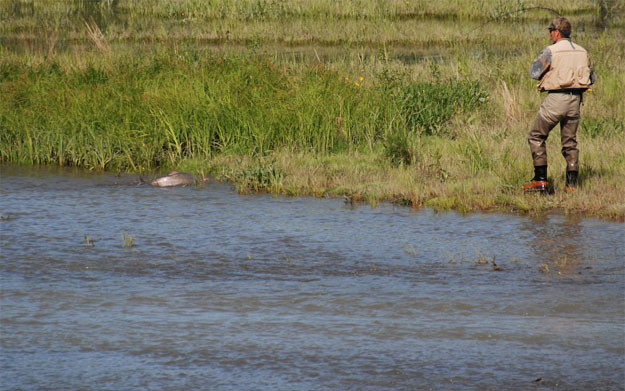
\includegraphics[width=\textwidth]{images/evaluation/SeedsSantner/image_0011_9060}
\caption{Image originale.}
 \end{subfigure}
 \\
 \begin{subfigure}[t]{0.4\textwidth}
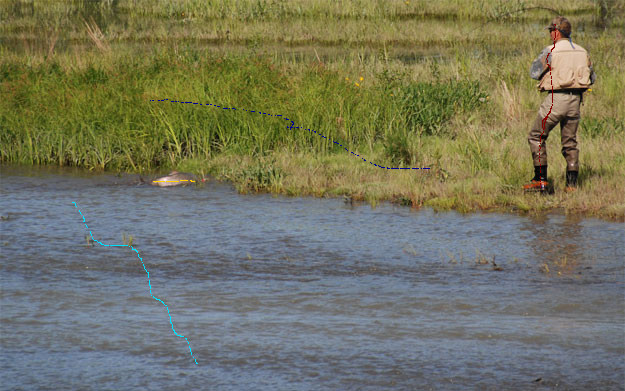
\includegraphics[width=\textwidth]{images/evaluation/SeedsSantner/image_0011_9060_seeds_santner}
\caption{Germes de Santner \textit{et al.}}
 \end{subfigure}
 ~
 \begin{subfigure}[t]{0.4\textwidth}
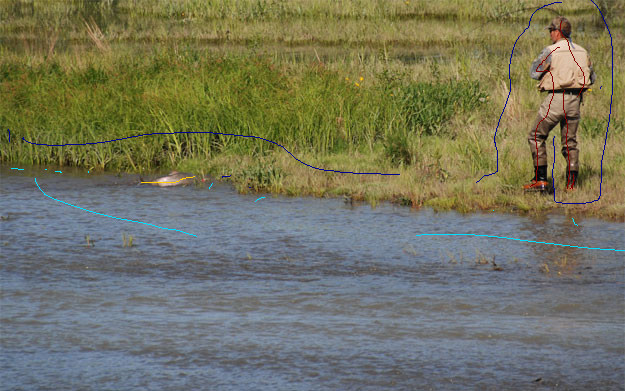
\includegraphics[width=\textwidth]{images/evaluation/SeedsSantner/image_0011_9060_seeds_saf}
\caption{Germes donnés en demandant à l'utilisateur de \modif{donner des germes près des contours}.}
 \end{subfigure}
 \\
 \begin{subfigure}[t]{0.4\textwidth}	
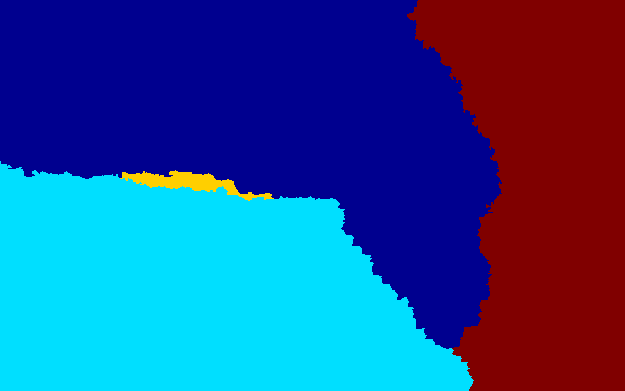
\includegraphics[width=\textwidth]{images/evaluation/SeedsSantner/image_0011_9060_seeds_santner_res}
\caption{Résultat \modif{de $S \alpha F$}  avec les germes de Santner \textit{et al.}}
 \end{subfigure}
 ~
 \begin{subfigure}[t]{0.4\textwidth}	
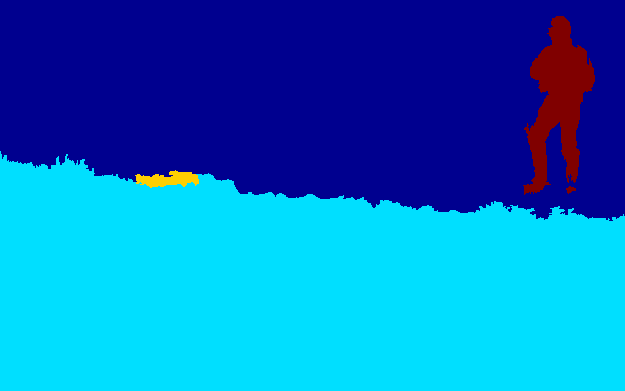
\includegraphics[width=\textwidth]{images/evaluation/SeedsSantner/image_0011_9060_seeds_saf_res}
\caption{Résultat \modif{de $S \alpha F$}  avec \modif{les} germes \modif{près des contours}.}
 \end{subfigure}
\caption{Illustration de l'un des cas où les germes de Santner \textit{et al.} ne conviennent pas à $S \alpha F$. Ici des germes \modif{plus nombreux} doivent être \modif{donnés} pour marquer les délimitations entre la rivière et l'herbe ainsi qu'entre l'herbe et le pêcheur. }
	\label{fig:eval:seedsSantner1}
\end{figure} 


\begin{figure}[htb]
 \centering
 \begin{subfigure}[t]{0.4\textwidth}	
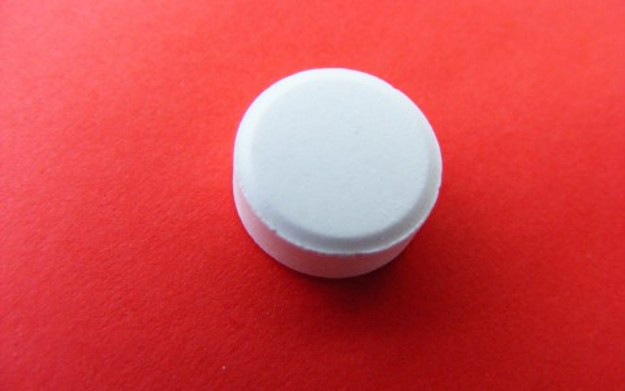
\includegraphics[width=\textwidth]{images/evaluation/SeedsSantner/image_0217_9060}
\caption{Image originale.}
 \end{subfigure}
 \\
 \begin{subfigure}[t]{0.4\textwidth}
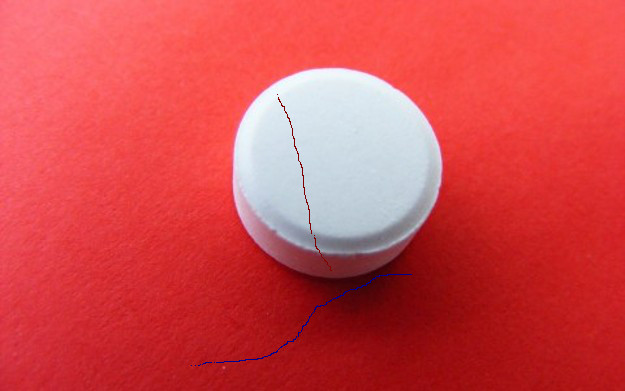
\includegraphics[width=\textwidth]{images/evaluation/SeedsSantner/image_0217_9060_seeds_santner}
\caption{Germes de Santner \textit{et al.}}
 \end{subfigure}
 ~
 \begin{subfigure}[t]{0.4\textwidth}
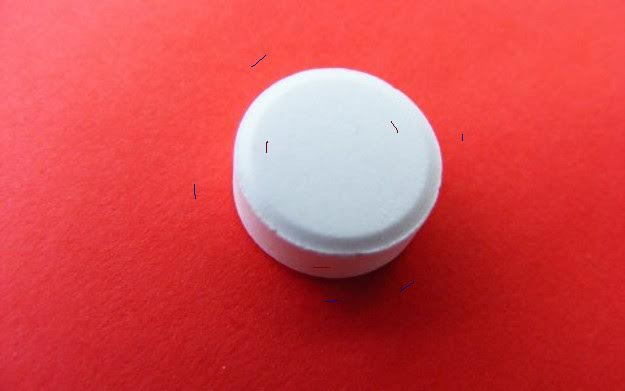
\includegraphics[width=\textwidth]{images/evaluation/SeedsSantner/image_0217_9060_seeds_saf}
\caption{Germes donnés en demandant à l'utilisateur de  \modif{donner des germes près des contours}.}
 \end{subfigure}
 \\
 \begin{subfigure}[t]{0.4\textwidth}	

\includegraphics[width=\textwidth]{images/evaluation/SeedsSantner/image_0217_9060_seeds_santner_res}
\caption{Résultat \modif{de $S \alpha F$} avec les germes de Santner \textit{et al.}}
 \end{subfigure}
 ~
 \begin{subfigure}[t]{0.4\textwidth}	

\includegraphics[width=\textwidth]{images/evaluation/SeedsSantner/image_0217_9060_seeds_saf_res}
\caption{Résultat \modif{de $S \alpha F$} avec \modif{les} germes \modif{près des contours}.}
 \end{subfigure}
\caption{Illustration de l'un des cas où les germes de Santner \textit{et al.} ne conviennent pas à $S \alpha F$. Ici, il n'est pas nécessaire d'ajouter davantage de germes : ils doivent seulement être positionnés \modif{différemment}. }
	\label{fig:eval:seedsSantner2}
\end{figure} 
\subsubsection{\modif{Tests avec de nouveaux germes}}
 
Nous avons effectué des tests supplémentaires  avec deux ensembles de germes, \modif{différents de ceux de Santner \textit{et al.} \cite{santner2010interactive}} :
\begin{itemize}
\item ${S \alpha F_{0} }$, l'ensemble des germes initiaux, donnés avant que l'utilisateur ne voit le résultat de l'étape de segmentation ;
\item $S \alpha F_{N}$, l'ensemble des germes corrigés par l'utilisateur, \modif{correspondant donc à la dernière itération)}, afin que la segmentation produite soit la plus proche possible de la segmentation de référence.
\end{itemize}

À l'instar des germes de Santner \textit{et al.} \cite{santner2010interactive}, les germes de ${S \alpha F_{0} }$ ont été \modif{obtenus} sans permettre à l'utilisateur de voir le résultat de la segmentation et de s'en servir pour guider la méthode. Cependant, une consigne supplémentaire a été \modif{donnée} à ce dernier : donner des germes initiaux proches des contours des objets.

Avec les germes ${S \alpha F_{0} }$ et les images de Santner \textit{et al.}, $S \alpha F$ obtient une score \modif{$\mathcal{F}_{DICE}$} moyen de \modif{$97$}. En permettant à l'utilisateur d'enlever ou d'ajouter des germes afin de corriger les erreurs commises par $S \alpha F$ (ce qui correspond aux germes de l'ensemble $S \alpha F_{N}$) ce score \modif{passe} à \modif{$98$}. Les erreurs restantes proviennent de l'étape de sur-segmentation et ne peuvent généralement pas être \modif{corrigées}. 

Le temps d'exécution moyen par image est de $\nombre{1,2}$ seconde. Celui des méthodes de Santner \textit{et al.} et de \modif{Müller} \textit{et al.} avoisine les \modif{$2$} secondes. Cependant, alors que ces deux algorithmes reposent sur une implémentation tirant parti de la puissance de calcul d'une carte graphique, $S \alpha F$ n'a fait l'objet d'aucune optimisation particulière et ne nécessite pas une configuration matérielle spécifique. Nous verrons dans la section \ref{subsec:eval:opp}  que cette faible complexité permet d'utiliser $S \alpha F$ au sein d'une application mobile.


Ces résultats nous permettent de conclure que $S \alpha F$, malgré la contrainte qu'il impose au niveau des germes, est une méthode compétitive par rapport à celles de Santner \textit{et al.} et de \modif{Müller} \textit{et al.}

\begin{emodif}
Quelques autres exemples de segmentations produites par $S \alpha F$ pour les problèmes de segmentation \modif{multiclasse} de Santner \textit{et al.} sont donnés sur la figure \ref{fig:eval:ResST}.
\begin{figure}[htb]
	\centering	
	 \begin{subfigure}[B]{\textwidth}
	 \centering
			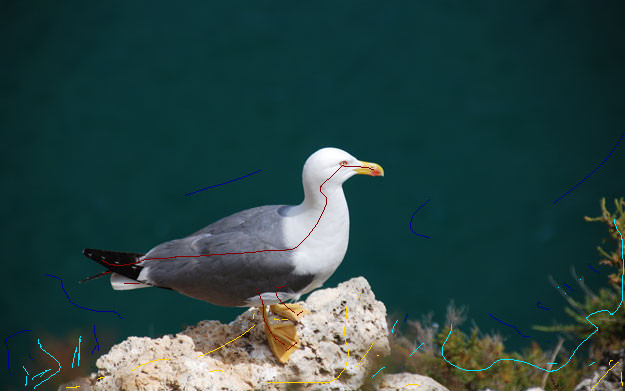
\includegraphics[width=0.45\textwidth]{images/evaluation/Santner/image_0015_seeds}
			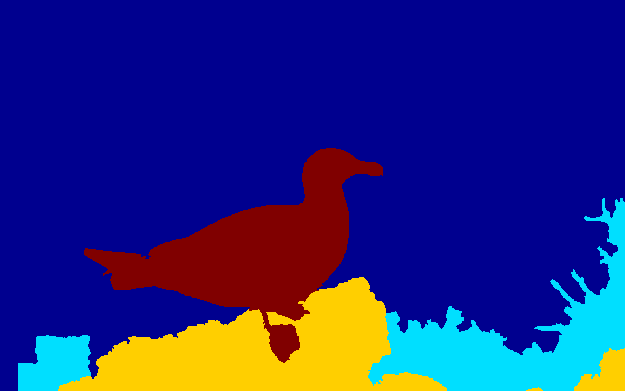
\includegraphics[width=0.45\textwidth]{images/evaluation/Santner/image_0015_seg}
		 \caption{Ici, peu de germes sont nécessaires pour segmenter correctement le fond de couleur unie. Les branchages, pourtant moins nets, sont également correctement extraits. Tandis que les contours du goéland sont réguliers et arrondis, ceux du rocher restituent la granularité de ce dernier.}
	\end{subfigure}		
	\\	
	 \begin{subfigure}[B]{\textwidth}	
	 \centering
			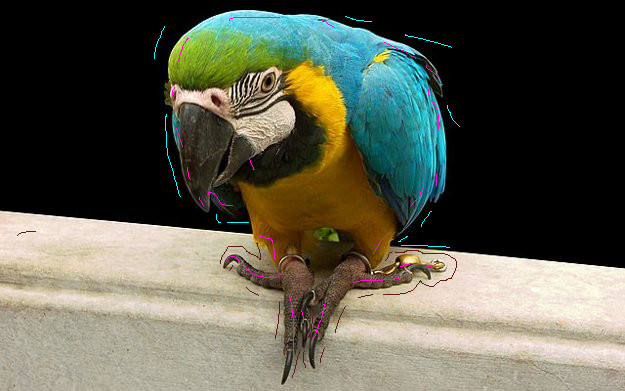
\includegraphics[width=0.45\textwidth]{images/evaluation/Santner/image_0236_seeds}
			
\includegraphics[width=0.45\textwidth]{images/evaluation/Santner/image_0236_seg}
		 \caption{Bien qu'ils constituent des détails de faible dimension, les ergots du perroquet sont correctement extraits. }
	\end{subfigure}	
	\\	
	 \begin{subfigure}[B]{\textwidth}	
	 \centering
			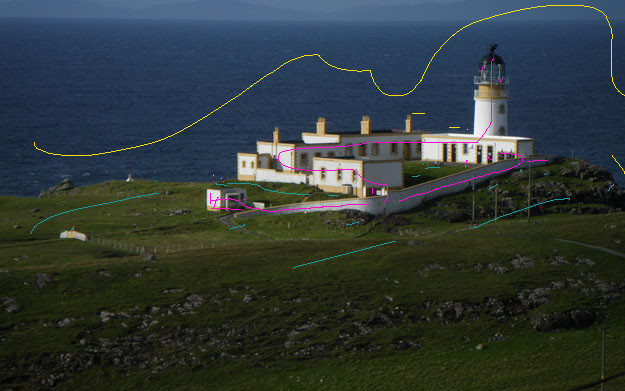
\includegraphics[width=0.45\textwidth]{images/evaluation/Santner/image_0030_seeds}
			
\includegraphics[width=0.45\textwidth]{images/evaluation/Santner/image_0030_seg}
		 \caption{Bien qu'il contienne des petits détails architecturaux, le bâtiment est correctement segmenté.}
	\end{subfigure}	
	\caption{Exemples de germes donnés et de résultats obtenus sur les données de référence de Santner \textit{et al.} \cite{santner2010interactive}.}
	\label{fig:eval:ResST}
\end{figure}
\end{emodif}


\subsection{Algorithme de Changjae \textit{et al.}}

\begin{emodif}

Changjae \textit{et al.}  \cite{Changjae2017Robust} ont évalué leur méthode sur les données de référence de Rother \textit{et al.} \cite{rother2004grabcut} ainsi que sur 50 images parmi les données de référence de Santner \textit{et al.} \cite{santner2010interactive}. Ils utilisent eux aussi des germes donnés manuellement, mais n'étant pas modifié par l'utilisateur. Comme ces germes n'ont pas été mis à disposition, une comparaison avec $S \alpha F$ est délicate.

Les scores $\mathcal{F}_{DICE}$  obtenus par l'algorithme de Changjae \textit{et al.}  \cite{Changjae2017Robust} sont, dans le meilleur des cas, de $93$ pour les données de Rother \textit{et al.} \cite{rother2004grabcut} et de $90$ sur les 50 images issues des données de référence de Santner \textit{et al.} \cite{santner2010interactive}. Sans permettre à l'utilisateur de modifier les germes, $S \alpha F$ améliore le score sur les données de Rother \textit{et al.} \cite{rother2004grabcut} de $3$ points. Comme nous ne connaissons pas les 50 images retenues parmi les données de Santner \textit{et al.}, nous ne pouvons pas tirer de conclusion, même si le score obtenu par $S \alpha F$ pour l'ensemble de ces données est de $97$, sans modification des germes. 

Le bénéfice le plus clair de $S \alpha F$ reste au niveau du temps d'exécution, significativement plus court : à peine plus d'une seconde pour $S \alpha F$, tandis que $40$ secondes sont nécessaires à la méthode Changjae \textit{et al.}  

\end{emodif}


\section{Bénéfice apporté par le terme de régularisation}

Afin d'analyser l'impact du terme de régularisation, nous avons conçu une version simplifiée de $S \alpha F$ \modif{qui, au lieu de la fonction décrite par l'équation \ref{eq:saf:eqgf}, minimise :}
\modif{
\begin{equation}
\mathcal{F}_{SCIS} (C, I) = \prod_{i=1}^{N_{I}} \exp( \mathcal{F}_{D}(x_{i},c_{i}) ) \text{.}
\end{equation}
}
Comme seul le terme d'attache aux données apparaît dans la fonction  $\mathcal{F}_{SCIS}$, la segmentation correspondant à son minimum est obtenue en attribuant à chaque superpixel la classe la plus probable, c'est-à-dire en utilisant directement \modif{la classe ayant la plus forte probabilité, selon l'approche de Wu \textit{et al.} \cite{wu2004probability}}.  Nous avons nommé cette variante $SCIS$, de l'anglais \modif{\og \emph{Superpixel Classification-based Interactive Segmentation}\fg}. 

Nous avons comparé $SCIS$ et $S \alpha F$ à partir des données de référence de Rother \textit{et al.}  \cite{rother2004grabcut}, de  McGuinness \textit{et al.} \cite{mcguinness2010comparative}  et de Santner \textit{et al. } \cite{santner2010interactive}. En donnant de nombreux germes, nous avons réussi à obtenir avec $SCIS$ :
\begin{itemize}
\item un score  \modif{$\mathcal{F}_{Jaccard}$} égal à celui de $S \alpha F$ pour les données de Rother \textit{et al.} ; 
\item des scores \modif{$\mathcal{F}_{Jaccard}$} et  \modif{$\mathcal{F}_{FCnt}$} identiques à ceux de $S \alpha F$ pour les données de McGuiness \textit{et al.} ;
\item  un score  \modif{$\mathcal{F}_{DICE}$} similaire pour les données de Santner \textit{et al.}
\end{itemize}

La complexité algorithmique de $SCIS$ est moins élevée que celle de $S \alpha F$. Ainsi, lors de l'étape d'initialisation, il n'est pas nécessaire d'estimer \modif{$P_{i}(j)$}, la probabilité pour un superpixel de classe de label $\lambda_{i}$ d'avoir comme voisin un superpixel attribué à la classe de label $\lambda_{j}$. Quant à l'étape de segmentation, elle ne nécessite pas d'utiliser l'algorithme $\alpha$-fusion. Néanmoins, cette simplicité se paie par un nombre de germes plus \modif{élevé}. 


\begin{table}[h]
\begin{center}
\begin{tabular}{| l | l | l | l | l |  l | l |}
\hline 
\cellcolor{gris}{Données}&  \multicolumn{2}{|c|}{\cellcolor{gris}Rother \textit{et al.}} &  \multicolumn{2}{|c|}{\cellcolor{gris}McGuinness \textit{et al.}} & \multicolumn{2}{|c|}{\cellcolor{gris}Santner \textit{et al.}}\\
\hline
&$SCIS$&$S \alpha F$&$SCIS$&$S \alpha F$&$SCIS$&$S \alpha F$\\
\hline
\cellcolor{gris}{Pr (\%)}&$\nombre{2,08} \pm \nombre{0,36}$&$\nombre{0,74} \pm \nombre{0,36}$ &$\nombre{2,08} \pm \nombre{0,49}$&$\nombre{1,26} \pm \nombre{0,69}$ &$\nombre{1,42} \pm \nombre{0,42}$&$\nombre{0,89} \pm \nombre{0,43}$\\
\hline
$\cellcolor{gris}{T_{init}\text{ (s)}} $&$\nombre{0,6} \pm \nombre{0,18}$&$\nombre{0,61} \pm \nombre{0,19}$& $\nombre{0,4} \pm \nombre{0,01}$&$\nombre{0,41} \pm \nombre{0,01}$ &$\nombre{0,64} \pm \nombre{0,02}$&$\nombre{0,66} \pm \nombre{0,02}$\\
\hline
$\cellcolor{gris}{T_{seg}\text{ (s)}}$&$\nombre{0,04} \pm \nombre{0,02}$&$\nombre{0,27} \pm \nombre{0,02}$&$\nombre{0,06} \pm \nombre{0,03}$&$\nombre{0,68} \pm \nombre{0,04}$ &$\nombre{0,06} \pm \nombre{0,04}$&$\nombre{0,51} \pm \nombre{0,28}$\\
\hline
\end{tabular}
\end{center}
\caption{Comparaison entre $SCIS$ et $S \alpha F$. Moyennes et écarts types pour le pourcentage de pixels annotés par l'utilisateur ($Pr$) ainsi que les temps d'exécution lors de l'étape d'initialisation ($T_{init}$) et de l'étape de segmentation ($T_{seg}$). Ces valeurs sont obtenues en produisant des segmentations dont la précision est similaire.}
\label{tab:eval:SCISEval}
\end{table}


Le tableau \ref{tab:eval:SCISEval} donne, pour chaque ensemble de données de référence et pour chaque méthode, le temps d'exécution pour l'étape d'initialisation, le temps d'exécution pour l'étape de segmentation et le pourcentage de pixels annotés par l'utilisateur\modif{, à l'issue de la dernière itération}. Ces résultats montrent que $SCIS$ nécessite environ  $1 \%$ de germes supplémentaires (ce pourcentage étant donné par rapport à l'ensemble des pixels de l'image). Concrètement, il s'agit de plus \modif{$200\ 000$}  pixels supplémentaires assignés à une classe par l'utilisateur. Ces germes doivent par ailleurs être répartis de manière beaucoup plus uniforme dans l'image en termes de localisation\modif{, et cela dans l'ensemble de l'image et pas uniquement près des contours}. La figure  \ref{fig:eval:seedsComparison} montre un exemple des différences entre les germes donnés pour $SCIS$ et ceux pour  $S \alpha F$. 

\begin{figure}[htb]
\centering
 \begin{subfigure}{0.4\textwidth}	
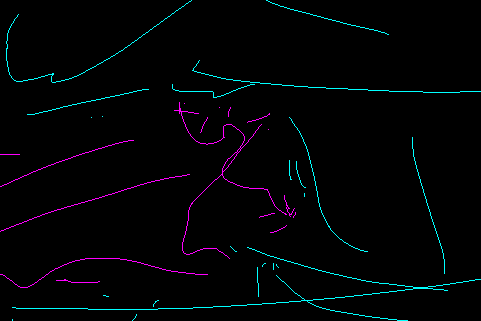
\includegraphics[width=\textwidth]{images/evaluation/seeds_SCIS}
		 \caption{Germes nécessaires à $SCIS$.}
 \end{subfigure}
 ~
 \begin{subfigure}{0.4\textwidth}	
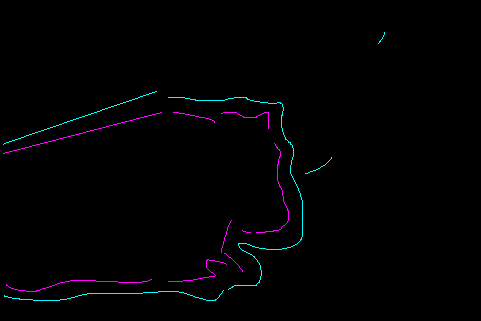
\includegraphics[width=\textwidth]{images/evaluation/seeds_SAF}
		 \caption{Germes nécessaires à $S \alpha F$.}
 \end{subfigure}
 \caption{Réduction du nombre de germes par \modif{l'utilisation} du terme de régularisation.}
 \label{fig:eval:seedsComparison}
\end{figure} 

Si la différence entre les germes à donner pour $S \alpha F$ et ceux nécessaires à $SCIS$ correspond à un effort nettement perceptible \modif{par} l'utilisateur, les variations en termes de temps d'exécution sont plus ténues. Elles concernent très peu l'étape d'initialisation : dans le pire des cas l'écart est de seulement $\nombre{0,02}$ seconde. Avec des images \modif{de grande taille}, il est cependant probable que la différence entre les deux méthodes se creuse, en faveur de $SCIS$. 

Pour l'étape de segmentation, la différence entre les durées est plus marquée. Néanmoins, la complexité de cette étape étant liée au nombre de superpixels et pas \modif{à la taille} de l'image, le fait d'augmenter le nombre de pixels ne \modif{la fait pas croître}. Comme nous le verrons dans la section suivante, le temps nécessaire à $S \alpha F$ pour segmenter l'image après avoir donné les germes reste autour de $\nombre{0,5}$ seconde, même en augmentant sensiblement la taille de l'image. 

Afin de conclure cette analyse, il convient de décrire un peu le fonctionnement de $S \alpha F$ tel \modif{qu'il est} perçu par l'utilisateur. L'étape d'initialisation ne nécessite pas la présence des germes et peut parfaitement être réalisé à l'insu de l'utilisateur, pendant que ce dernier est en train de sélectionner les germes. Lorsque l'utilisateur a terminé, la méthode termine si nécessaire l'initialisation et effectue, en moins d'une seconde, l'étape de segmentation. À partir de ce moment, seule l'étape de segmentation est répétée\modif{, tant que l'utilisateur modifie les germes}. 

En définitive, le temps passé par l'utilisateur à ajouter les germes nécessaires à $SCIS$ est nettement plus perceptible que la différence de temps d'exécution entre $SCIS$ et $S \alpha F$. L'\modif{utilisation} d'un terme de régularisation améliore donc l'ergonomie de $S \alpha F$.

\section{Passage à l'échelle}

\subsection{Protocole}
Afin d'analyser le passage à l'échelle de l'algorithme $S \alpha F$, nous avons créé, à partir des données de référence de HSID, trois nouveaux ensembles de référence \modif{$HSID'_{1}$}, \modif{$HSID'_{2}$} et \modif{$HSID'_{3}$}. Ils sont composés des mêmes images  mais à des tailles différentes. Chaque ensemble de référence comprend $50$ images. Les photographies de \modif{$HSID'_{1}$} contiennent $1800 \times 1201$ pixels. Celles de \modif{$HSID'_{2}$} ont été ramenées à $1350 \times 901$ de pixels et celles de \modif{$HSID'_{3}$} à $1013 \times 676$ pixels.  

Une unique segmentation de référence est associée à chaque image de chaque ensemble. \modif{Les segmentations de référence de $HSID'_{i-1}$ correspondent aux segmentations de référence de $HSID'_{i}$ dont les tailles ont été réduites. Lorsque cette réduction de la taille a engendré des erreurs, elles ont été corrigées manuellement. Les germes pour chaque ensemble ont été obtenu selon le même procédé, en partant des germes donnés pour $HSID'_{1}$.} 

Comme le montre la figure \ref{fig:eval:HSIDClasses}, le nombre de classes dans les segmentations se situent principalement entre $2$ et $4$ classes. \modif{Le nombre de classes est le même pour chacun des trois ensembles de données de référence.}

\begin{figure}[htb]
\begin{center}
\scalebox{.5}{
\input{images/evaluation/HSIDClasses.pdf_t}
}
\caption{Répartition du nombre de classes pour chaque ensemble de référence \modif{$HSID'_{i}$}.}
\label{fig:eval:HSIDClasses}
\end{center}
\end{figure}

Pour évaluer l'adéquation entre les segmentations produites par $S \alpha F$ et les segmentations de références nous avons utilisé la mesure $\mathcal{F}_{DICE}$. Nous nous sommes également intéressés au temps d'exécution \modif{de} l'étape d'initialisation et \modif{de} l'étape de segmentation. Nous avons \modif{calculé} la valeur moyenne, l'écart type, le minimum et le maximum de ces trois mesures, pour \modif{chacun} des trois ensembles de référence.

Enfin, durant l'ensemble de nos tests, nous n'avons pas modifié les paramètres. En particulier, toutes les images sont sur-segmentées en $3000$ superpixels environ.

\subsection{Analyse des résultats}

Les résultats obtenus par $S \alpha F$ sont présentés dans :
\begin{itemize}
\item le tableau \ref{tab:eval:Algo-Scalability-Dice}, pour le score $\mathcal{F}_{DICE}$ ;
\item le tableau \ref{tab:eval:Algo-Scalability-Init-Time}, pour \modif{le} temps d'exécution lors de l'étape d'initialisation ;
\item le tableau \ref{tab:eval:Algo-Scalability-Seg-Time}, pour \modif{le} temps d'exécution lors de l'étape de segmentation.
\end{itemize} 

\begin{table}[h]
\centering
\begin{tabular}{|l|l|l|l| }
\hline 
\cellcolor{gris}{Données}&\cellcolor{gris}{Moyenne $\pm$ écart type}&\cellcolor{gris}{Minimum}&\cellcolor{gris}{Maximum}\\
\hline
\modif{$HSID'_{3}$}&$99\% \pm \nombre{1,03}$ & \modif{$95$}  & \modif{$100$}\\
\hline
\modif{$HSID'_{2}$}&$99\% \pm \nombre{0,99}$ & \modif{$95$}  & \modif{$100$}\\
\hline
\modif{$HSID'_{1}$}&$99\% \pm \nombre{1,12}$ & \modif{$95$} & \modif{$100$}\\
\hline
\end{tabular}
\caption{Valeurs de la mesure $\mathcal{F}_{DICE}$ obtenues par $S \alpha F$.}
\label{tab:eval:Algo-Scalability-Dice}
\end{table}

L'analyse de l'adéquation entre les segmentations produites et les segmentations de référence montre que la qualité des résultats de $S \alpha F$ n'est pas influencée par l'augmentation ou la diminution des dimensions de l'image. L'écart type relativement faible, ainsi que la différence ténue (seulement $5\%$) entre la valeur \modif{minimale} et la valeur \modif{maximale}, indiquent par ailleurs que les performances de $S \alpha F$ demeurent stables, quelle que soit la segmentation de référence à atteindre.


\begin{table}[h]
\centering
\begin{tabular}{|l|l|l|l| }
\hline
\cellcolor{gris}{Données}&\cellcolor{gris}{Moyenne $\pm$ écart type}&\cellcolor{gris}{Minimum}&\cellcolor{gris}{Maximum}\\
\hline
\modif{$HSID'_{3}$}&$\nombre{1,79} \pm \nombre{0,06}$ & $\nombre{1,71} $ & $\nombre{1,98}$\\
\hline
\modif{$HSID'_{2}$}&$\nombre{3,25} \pm \nombre{0,12}$ & $\nombre{3,06} $ & $\nombre{3,64}$\\
\hline
\modif{$HSID'_{1}$}&$\nombre{5,73} \pm \nombre{0,25}$ & $\nombre{5,34} $ & $\nombre{6,33}$\\
\hline
\end{tabular}
\caption{Temps \modif{d’exécution} de $S \alpha F$ (en secondes) lors de l'étape d'initialisation.}
\label{tab:eval:Algo-Scalability-Init-Time}
\end{table}
 
\begin{table}[h]
\centering
\begin{tabular}{|l|l|l|l| }
\hline 
\cellcolor{gris}{Données}&\cellcolor{gris}{Moyenne $\pm$ écart type}&\cellcolor{gris}{Minimum}&\cellcolor{gris}{Maximum}\\
\hline
\modif{$HSID'_{3}$}&$\nombre{0,46} \pm \nombre{0,28}$ & $\nombre{0,21} $ & $\nombre{1,64}$\\
\hline
\modif{$HSID'_{2}$}&$\nombre{0,46} \pm \nombre{0,28}$ & $\nombre{0,21} $ & $\nombre{1,68}$\\
\hline
\modif{$HSID'_{1}$}&$\nombre{0,41} \pm \nombre{0,22}$ & $\nombre{0,2} $ & $\nombre{1,2}$\\
\hline
\end{tabular}
\caption{Temps \modif{d’exécution} de $S \alpha F$ (en secondes) lors de l'étape de segmentation.}
\label{tab:eval:Algo-Scalability-Seg-Time}
\end{table}

Le résultat le plus intéressant de cette évaluation concerne les temps d'exécution pour chacune des deux étapes. Tandis que le temps nécessaire pour l'initialisation augmente avec le nombre de pixels, la durée de la phase de segmentation demeure stable et en dessous de la seconde. Or, l'étape d'initialisation ne nécessite pas la présence des germes. Elle peut donc être réalisée avant ou pendant que l'utilisateur les donne. Le temps perçu est alors réduit à la seule durée de la segmentation, permettant à l'utilisateur de percevoir une très bonne réactivité de $S \alpha F$.

Ce résultat est tout à fait cohérent, puisque l'étape d'initialisation travaille à l'échelle du pixel tandis que l'étape de segmentation manipule les superpixels. Or, si le nombre de pixels augmente avec \modif{la taille} de l'image, le nombre de superpixels, lui, ne varie pas. La figure \ref{fig:eval:ResHSID} donne quelques exemples des germes utilisés et des segmentations obtenues sur \modif{$HSID'_{2}$}.


\begin{figure}[htb]
	\centering	
	 \begin{subfigure}[B]{\textwidth}
	 \centering
			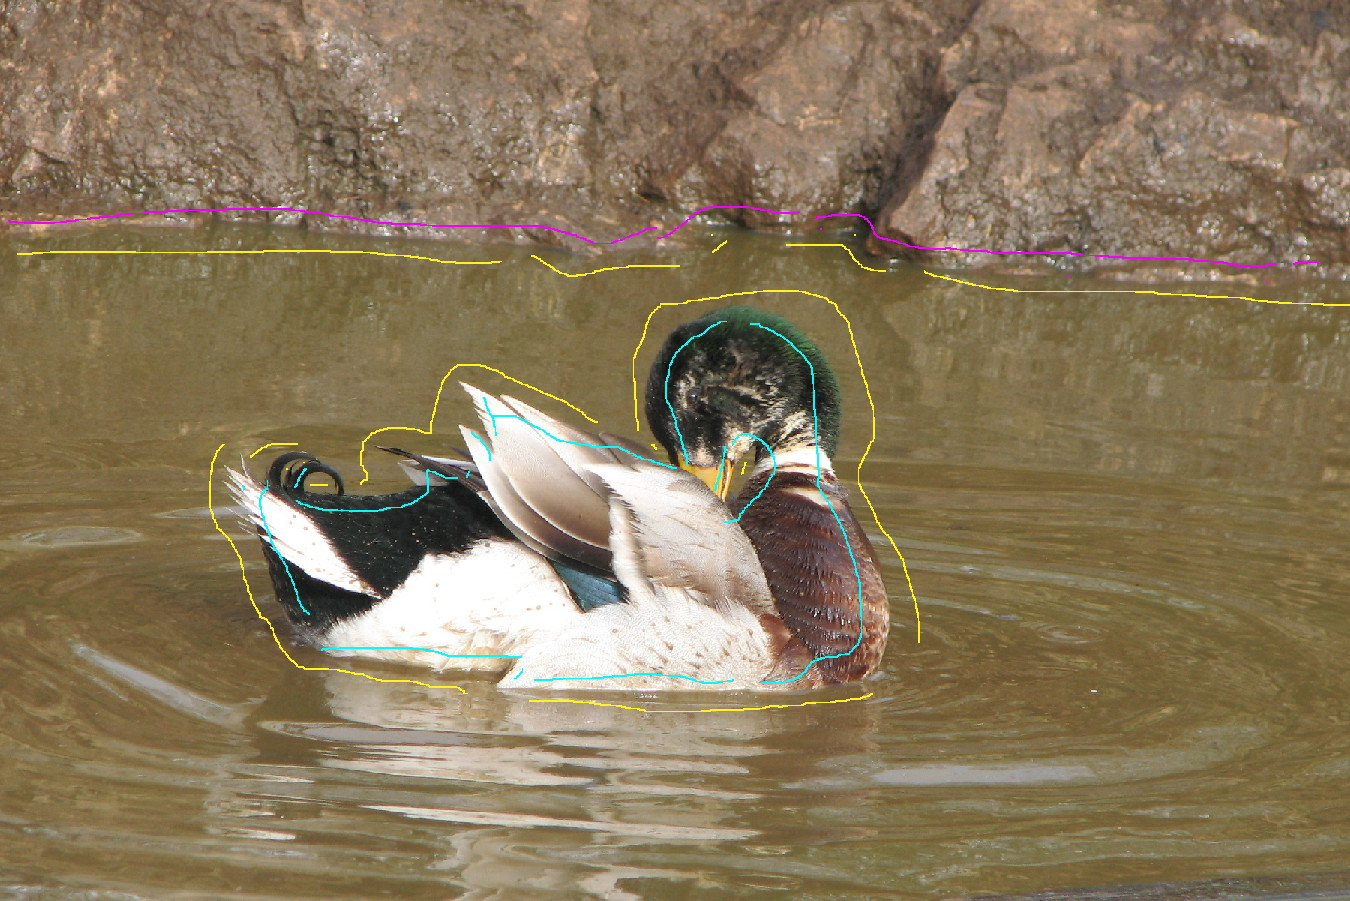
\includegraphics[width=0.45\textwidth]{images/evaluation/HSID/img_5_seeds}
			
\includegraphics[width=0.45\textwidth]{images/evaluation/HSID/img_5_seg}
		 \caption{Le faible contraste entre l'eau et la pierre n'empêche pas de séparer ces deux éléments.}
	\end{subfigure}		
	\\	
	 \begin{subfigure}[B]{\textwidth}	
	 \centering
			\includegraphics[width=0.45\textwidth]{images/evaluation/HSID/img_12_seeds}
			\includegraphics[width=0.45\textwidth]{images/evaluation/HSID/img_12_seg}
		 \caption{Utiliser des superpixels n'empêche pas de segmenter avec précision la fourrure du glouton. Quelques erreurs sont cependant \modif{visibles} au niveau de la patte avant \modif{gauche} dont la couleur se confond avec l'ombre. Ces erreurs sont commises au niveau des superpixels et ne peuvent \modif{pas} être \modif{corrigées} même en ajoutant des germes.} 
	\end{subfigure}	
	\caption{Exemples de germes donnés et de résultats obtenus sur l'ensemble de référence \modif{$HSID'_{2}$}.}
	\label{fig:eval:ResHSID}
\end{figure}

\section{Ergonomie}
\label{sec:eval:ergonomie}

\subsection{Problématique}
Les questionnaires pour les utilisateurs réalisés et analysés par McGuinness \textit{et al.} \cite{mcguinness2010comparative} montrent que, pour qu'une méthode de segmentation interactive soit reçue favorablement, il ne lui suffit pas de permettre la production rapide d'une segmentation précise : il est également essentiel que l'utilisateur, même néophyte, comprennent rapidement comment positionner les germes pour arriver au résultat souhaité. Ainsi, même si l'algorithme de Salembier \textit{et al.} \cite{salembier2000binary} obtient un meilleur score d'adhérence aux contours que celui de Boykov \textit{et al.} \cite{boykov2001interactive}, c'est ce dernier que les utilisateurs plébiscitent.

Par sa structure, la méthode de Boykov \textit{et al.} favorise un impact local des germes : en particulier, ajouter des germes à un endroit de la photographie n'influe pas\modif{,} ou très peu\modif{,} le reste de la segmentation.
Nous nous sommes appuyés sur ce résultat lors de la conception de $S \alpha F$, notamment en choisissant d'introduire une information de localisation dans le descripteur afin de tempérer l'influence de l'information de couleur. Cette caractéristique, en plus d'être nécessaire à la séparation de deux objets similaires (comme les porcelets de la figure \ref{fig:eval:MgDBEx}b), permet de retrouver l'influence locale des indications données qui fait la force de l'algorithme de Boykov \textit{et al.}


\subsection{Quelques études qualitatives}

Les figures \ref{fig:eval:Algo-predictability-1}, \ref{fig:eval:Algo-predictability-2} et \ref{fig:eval:Algo-predictability-3} montrent l'impact de l'ajout de germes sur les segmentations produites par $S \alpha F$ pour trois images.

L'analyse de ces trois figures montre qu'une première segmentation relativement proche de la segmentation de référence peut presque toujours être obtenue en positionnant les germes près de la bordure interne des objets à extraire, ce qui constitue une indication relativement simple à transmette à l'utilisateur. Cette caractéristique de $S \alpha F$ est liée à l'utilisation d'un SVM, un point près de la bordure d'un objet ayant davantage de chance de constituer un vecteur de support au sens de l'information de localisation.

Cette première segmentation comprend toutefois quelques erreurs. Afin de les corriger, il suffit d'ajouter de nouveaux germes sur les zones erronées. Les exemples présentés couvrent deux itérations de $S \alpha F$. Le fait que l'utilisateur puisse identifier d'un simple coup d’œil les zones erronées et qu'en positionnant des germes sur ces dernières, ces erreurs soient corrigées sans dégrader la segmentation des autres parties de l'image, constitue un point de fort de $S \alpha F$, à la fois parce que son comportement est facilement prévisible et parce qu'il reste intuitif pour l'utilisateur.

À l'issue de la troisième étape, la segmentation obtenue est quasiment similaire à la segmentation souhaitée. Les erreurs résiduelles sont dues à l'étape de sur-segmentation et ne peuvent pas être corrigées par l'ajout de germes.

\begin{figure}[htb]
 \centering
 \begin{subfigure}{0.4\textwidth}	
\includegraphics[width=\textwidth]{images/evaluation/118035.jpg}
 \end{subfigure}
 \\
 \begin{subfigure}{0.4\textwidth}	
\includegraphics[width=\textwidth]{images/evaluation/118035_seeds1.jpg}
 \end{subfigure}
 ~
 \begin{subfigure}{0.4\textwidth}	
\includegraphics[width=\textwidth]{images/evaluation/118035_res1.jpg}
 \end{subfigure}
 \\
 \begin{subfigure}{0.4\textwidth}	
\includegraphics[width=\textwidth]{images/evaluation/118035_seeds2.jpg}
 \end{subfigure}
 ~
 \begin{subfigure}{0.4\textwidth}	
\includegraphics[width=\textwidth]{images/evaluation/118035_res2.jpg}
 \end{subfigure}
 \\
 \begin{subfigure}{0.4\textwidth}	
\includegraphics[width=\textwidth]{images/evaluation/118035_seeds3.jpg}
 \end{subfigure}
 ~
 \begin{subfigure}{0.4\textwidth}	
\includegraphics[width=\textwidth]{images/evaluation/118035_res3.jpg}
 \end{subfigure}
\caption{Évolutions concomitantes des germes donnés et des segmentations produites par $S \alpha F$ sur un problème de binarisation issu des données de référence de McGuinness \textit{et al.} \cite{mcguinness2010comparative}. }
	\label{fig:eval:Algo-predictability-1}
\end{figure} 

\begin{figure}[htb]
 \centering
 \begin{subfigure}{0.4\textwidth}	
\includegraphics[width=\textwidth]{images/evaluation/004.jpg}
 \end{subfigure}
 \\
 \begin{subfigure}{0.4\textwidth}	
\includegraphics[width=\textwidth]{images/evaluation/004_seeds1.jpg}
 \end{subfigure}
 ~
 \begin{subfigure}{0.4\textwidth}	
\includegraphics[width=\textwidth]{images/evaluation/004_res1.jpg}
 \end{subfigure}
 \\
 \begin{subfigure}{0.4\textwidth}	
\includegraphics[width=\textwidth]{images/evaluation/004_seeds2.jpg}
 \end{subfigure}
 ~
 \begin{subfigure}{0.4\textwidth}	
\includegraphics[width=\textwidth]{images/evaluation/004_res2.jpg}
 \end{subfigure}
 \\
 \begin{subfigure}{0.4\textwidth}	
\includegraphics[width=\textwidth]{images/evaluation/004_seeds3.jpg}
 \end{subfigure}
 ~
 \begin{subfigure}{0.45\textwidth}	
\includegraphics[width=\textwidth]{images/evaluation/004_res3.jpg}
 \end{subfigure}
\caption{Évolutions concomitantes des germes donnés et des segmentations produites par $S \alpha F$ sur un problème à $4$ classes issu des données de référence \modif{$HSID'_{1}$}.}
	\label{fig:eval:Algo-predictability-2}
\end{figure} 

\begin{figure}[htb]
 \centering
 \begin{subfigure}{0.4\textwidth}	
\includegraphics[width=\textwidth]{images/evaluation/010.jpg}
 \end{subfigure}
 \\~\\
 \begin{subfigure}{0.4\textwidth}	
\includegraphics[width=\textwidth]{images/evaluation/010_seeds1.jpg}
 \end{subfigure}
 ~
 \begin{subfigure}{0.4\textwidth}	
\includegraphics[width=\textwidth]{images/evaluation/010_res1.jpg}
 \end{subfigure}
 \\~\\
 \begin{subfigure}{0.4\textwidth}	
\includegraphics[width=\textwidth]{images/evaluation/010_seeds2.jpg}
 \end{subfigure}
 ~
 \begin{subfigure}{0.4\textwidth}	
\includegraphics[width=\textwidth]{images/evaluation/010_res2.jpg}
 \end{subfigure}
 \\~\\
 \begin{subfigure}{0.4\textwidth}	
\includegraphics[width=\textwidth]{images/evaluation/010_seeds3.jpg}
 \end{subfigure}
 ~
 \begin{subfigure}{0.4\textwidth}	
\includegraphics[width=\textwidth]{images/evaluation/010_res3.jpg}
 \end{subfigure}
\caption{Évolutions concomitantes des germes donnés et des segmentations produites par $S \alpha F$ sur un problème à $4$ classes issu des données de référence \modif{$HSID'_{1}$}.}
	\label{fig:eval:Algo-predictability-3}
\end{figure} 


\section{Applications}
 
\subsection{Greffon pour le logiciel de manipulation d'images Gimp}

Le logiciel de manipulation d'images Gimp\footnote{\url{http://www.gimp.org/}} est une alternative gratuite et libre à Photoshop\footnote{\url{http://www.photoshop.com/}} qui offre aux utilisateurs un panel d'outils pour modifier leurs photographies. Si ces opérations peuvent rester légères (redresser l'image, réduire le bruit, augmenter le contraste), Gimp permet également de réaliser des manipulations complexes, en appliquant des traitements spécifiques à certaines parties d'une image ou en prélevant des extraits de différentes \modif{images} et en les organisant à la manière d'un collage. Les outils de sélection sont donc une composante essentielle du logiciel Gimp. Actuellement ils prennent cinq formes :
\begin{itemize}
\item des outils réalisant des sélections à l'aide de formes géométriques simples (rectangle, ellipse, polygone) ;
\item un outil sélectionnant tous les pixels d'une même couleur ;
\item un outil de binarisation interactive par recherche des contours, qui correspondant à l'implémentation de l'algorithme de Mortensen \textit{et al. }  \cite{mortensen1995intelligent} ;
\item un outil de binarisation interactive par recherche des régions, qui est une implémentation de l'algorithme de Friedland \textit{et al.} \cite{friedland2005siox}.
\end{itemize}

L'algorithme $S \alpha F$, implémenté comme greffon pour le logiciel Gimp, vient compléter ces outils. En effet, nous avons montré qu'il assure une sélection plus précise que les méthodes de Mortensen \textit{et al. }  \cite{mortensen1995intelligent}  et de Friedland \textit{et al.} \cite{friedland2005siox}. Par ailleurs, alors que ces deux algorithmes se contentent de produire des binarisations, $S \alpha F$ offre la possibilité de sélectionner en \modif{une} seule passe plusieurs objets. 


La figure \ref{fig:eval:saf-in-gimp} illustre le fonctionnement de $S \alpha F$ intégré au logiciel Gimp. Cet exemple part d'une image (figure \ref{fig:eval:saf-in-gimp}a)  souffrant d'un faible contraste et d'un peu de flou. Nous souhaitons faire intervenir trois retouches locales pour l'améliorer :
\begin{itemize}
\item nous voudrions colorer le ciel en rose et orangé, afin de donner un effet de coucher de soleil ;
\item au niveau des bâtiments, nous aimerions renforcer le contraste ; 
\item nous souhaiterions augmenter le contraste du canal et le colorer \modif{avec des teintes ambrées} afin de faire apparaître les reflets de l'eau.
\end{itemize}

\begin{figure}[htb]
 \centering
 \begin{subfigure}{0.6\textwidth}	
\includegraphics[width=\textwidth]{images/evaluation/img_manipulation_original}
\caption{Image originale.}
 \end{subfigure}
 \\
 \begin{subfigure}{0.45\textwidth}	
\includegraphics[width=\textwidth]{images/evaluation/img_manipulation_germes}
\caption{Germes.}
 \end{subfigure}
 ~
 \begin{subfigure}{0.45\textwidth}	
\includegraphics[width=\textwidth]{images/evaluation/img_manipulation_seg}
\caption{Segmentation obtenue. }
 \end{subfigure}
 \\
 \begin{subfigure}{0.6\textwidth}	
\includegraphics[width=\textwidth]{images/evaluation/img_manipulation_res}
\caption{Image modifiée.}
 \end{subfigure}
\caption{Utilisation de $S \alpha F$ comme greffon pour le logiciel Gimp.}
	\label{fig:eval:saf-in-gimp}
\end{figure} 


La figure \ref{fig:eval:saf-in-gimp}b montre les germes que nous avons fournis à $S \alpha F$ et la figure \ref{fig:eval:saf-in-gimp}c la segmentation obtenue. Les germes et le résultat sont donnés sur des \emph{calques} qui viennent se superposer à l'image originale sans en modifier les caractéristiques. En sélectionnant, par exemple, toute la zone bleue sur le calque de la segmentation et en basculant sur le calque contenant l'image originale, il est  possible d'appliquer un traitement local sur tous les pixels du ciel. La figure \ref{fig:eval:saf-in-gimp}c correspond à l'image modifiée.

\subsection{Observatoire\modif{s} photographique\modif{s} du paysage}
\label{subsec:eval:opp}

Traité du Conseil de l'Europe adopté en octobre 2000, la Convention Européenne du Paysage vise à mieux prendre en compte et préserver les paysages. Elle est à l'origine de la mise en place de nombreux observatoires photographiques du paysage\footnote{\modif{Deux exemples : \url{http://observatoiredespaysages.fr}, \url{http://www.paysages-citoyens.be}}}. Ces derniers consistent en une sélection de plusieurs lieux représentatifs d'une thématique (évolution du paysage après un chantier d'autoroute, zones \modif{périurbaines}, etc.) qui seront photographiés à intervalle de temps régulier (par exemple tous les mois) selon un protocole rigoureux garantissant que les images de la même série correspondront au même point de vue.


L'algorithme $S \alpha F$ a été intégré au sein d'une application distribuée, afin de faciliter la mise à jour et l'enrichissement d'un observatoire photographique. Cette application se compose d'une partie serveur (en PHP)\modif{,} permettant la consultation et la comparaison de photographies\modif{,} et d'un logiciel mobile, développé pour le système d'exploitation Android. L'application mobile gère la re-photographie des sites choisis. En particulier l'utilisateur peut :
\begin{itemize}
\item localiser le site à \modif{re-}photographier le plus proche ;
\item disposer d'une image guide qui facilite la rephotographie ;
\item créer une segmentation sémantique associée à la photographie prise \modif{en indiquant,} pour chaque pixel\modif{,} à quel type d'élément paysager il appartient (ciel, végétation, bâtiment, etc.).
\end{itemize}
Cette dernière étape est réalisée grâce à $S \alpha F$. La puissance de calcul et les ressources mémoire d'un smartphone étant limitées, $S \alpha F$ a fait l'objet d'une implémentation optimisée où l'étape d'initialisation est réalisée dès que la photographie est prise, pendant que l'utilisateur donne les premiers germes. Ainsi, seule la durée nécessaire à l'étape de segmentation est perçue par l'utilisateur, ce qui réduit considérablement le temps d'attente de ce dernier.

L'intérêt du dispositif, tant sur le plan géographique que sur le plan éducatif, \modif{a} fait l'objet d'une publication \cite{puel2017une} et d'une présentation lors des \emph{Journées Géomatique, Enseignement et Apprentissage} \modif{qui sont déroulées à Toulouse en janvier 2017}.

\section{Conclusions et perspectives} 

Analyser l'apport de l'algorithme $S \alpha F$ par rapport à l'état de l'art est une tâche délicate, les conditions d'évaluation de certaines méthodes n'étant pas reproductibles. Nous avons néanmoins montré que notre méthode est compétitive par rapport à l'état de l'art. 

Nous nous sommes ensuite intéressés à certaines propriétés de $S \alpha F$. Nous avons montré l'importance de l'\modif{utilisation} d'un terme de régularisation ainsi que les bénéfices de l'utilisation d'une méthode de sur-segmentation, lorsque des images de taille importante sont traitées. Enfin, nous avons abordé la question de l'ergonomie de $S \alpha F$ et notamment les particularités des germes à lui fournir.

La piste qui nous paraît actuellement la plus prometteuse pour améliorer $S \alpha F$ concerne l'étape de sur-segmentation. Tout d'abord, les erreurs commises par rapport aux segmentations de référence proviennent en majorité de cette étape. Les réduire augmenterait la précision des segmentations produites. Ensuite, le fait que les superpixels  ne contiennent, par construction, pas d'information de texture annihile les bénéfices que nous pourrions retirer à utiliser un descripteur un peu plus complexe, qui faciliterait sans doute la phase d'apprentissage des caractéristiques visuelles de chaque classe et se traduirait  par une réduction du nombre de germes nécessaires. Enfin, réduire le nombre de superpixels permettrait de gagner encore un peu plus de temps lors de l'étape de segmentation de $S \alpha F$. \modif{Le chapitre suivant constitue un premier pas dans la direction d'une nouvelle méthode de sur-segmentation prenant en compte ces pistes d'amélioration.}
